\chapter{Ontologies on the Web---putting it all together}
\label{ch14}

A comprehensive listing of ontologies in the wild is impossible, just as
a complete listing of all web pages is impossible. New ontologies and
open data sets on the Semantic Web are showing up every day. In Chapter~\ref{ch10}, we got a glimpse of the data sets that make up the data.gov project,
and we saw how data based on FOAF and OGP are scattered all over the
Web. In selecting ontologies for this chapter, we had to leave some
favorite projects behind.

We ended up with three examples. These examples were chosen for this
chapter because of their advanced use modeling features beyond
RDFS-Plus, and how widespread their impact has been.

The first is called Good Relations (GR for short). GR allows businesses
to make very detailed descriptions of their offerings on the
marketplace. GR is similar to the OGP model described in Chapter~\ref{ch10} in
that it provides a controlled vocabulary that can be used by Web content
providers to mark up web pages. It differs from OGP in that it has a
great deal more structure---business offerings come in all shapes and
sizes and have a lot of details describing them.

The second is called Quantities/Units/Dimensions/Types, or QUDT for
short. It addresses an obvious problem that must be solved in any
attempt to align quantitative data, that is, data from
multiple sources will be expressed in different units. In order to
integrate data, it is necessary to be able to determine whether two
quantities are commensurate (that's where the dimensions come in), and
if so, how to convert from one system to another (that's where the units
come in).

The third ontology is actually a whole collection of ontologies that are
collectively known as the Open Biological and Biomedical Ontologies
(OBO). As the name implies, this is a set of ontologies about biological
and biomedical information. In contrast to Good Relations, which is a
small vocabulary for describing information on the Web, OBO includes
massive amounts of data about biomedicine and biology, including genome
information, catalogs of known cancer genes, and biochemistry data.

\section{The Good Relations Ontology}

The Good Relations ontology (GR) was developed by Martin Hepp of the
E-Business and Web Science Research Group at the Universitaet der
Bundeswehr Muenchen. Like OGP, it has been used to annotate a large
number of web pages. Within a year of its release, already tens of
thousands of web pages were annotated in RDFa using GR. These
annotations have been used by search engines (Yahoo! and Google, in
particular) for Search Engine Optimization; the more completely a
product can be described, the more highly it can be trusted to be an
appropriate match for a search engine query. The use of GR for
annotating product web pages at Best Buy and overstock.com resulted in
web pages that were ranked more highly in search results than much more
established pages. But Good Relations can do more than simply give pages
a higher rank--- Google uses Good Relations data to enhance the
information it gives about a product in response to a search. Figure
13.1 shows search results for a product, with and without Good Relations
markup. The page with Good Relations markup provides much more
information to lead a potential buyer to the product.

How does GR allow someone to make such detailed descriptions of their
business? While GR is relatively simple (in comparison, say, to OBO),
there is more to it than can be covered in this case study. The
interested reader is encouraged to see more of the GR at
\href{http://purl.org/goodrelations/}{{http://purl.org/goodrelations/}}
for a full and current description of the ontology. We will cover just
enough of the GR ontology to see how it is used to describe products for
Search Engine Optimization.

\begin{figure}
\centering
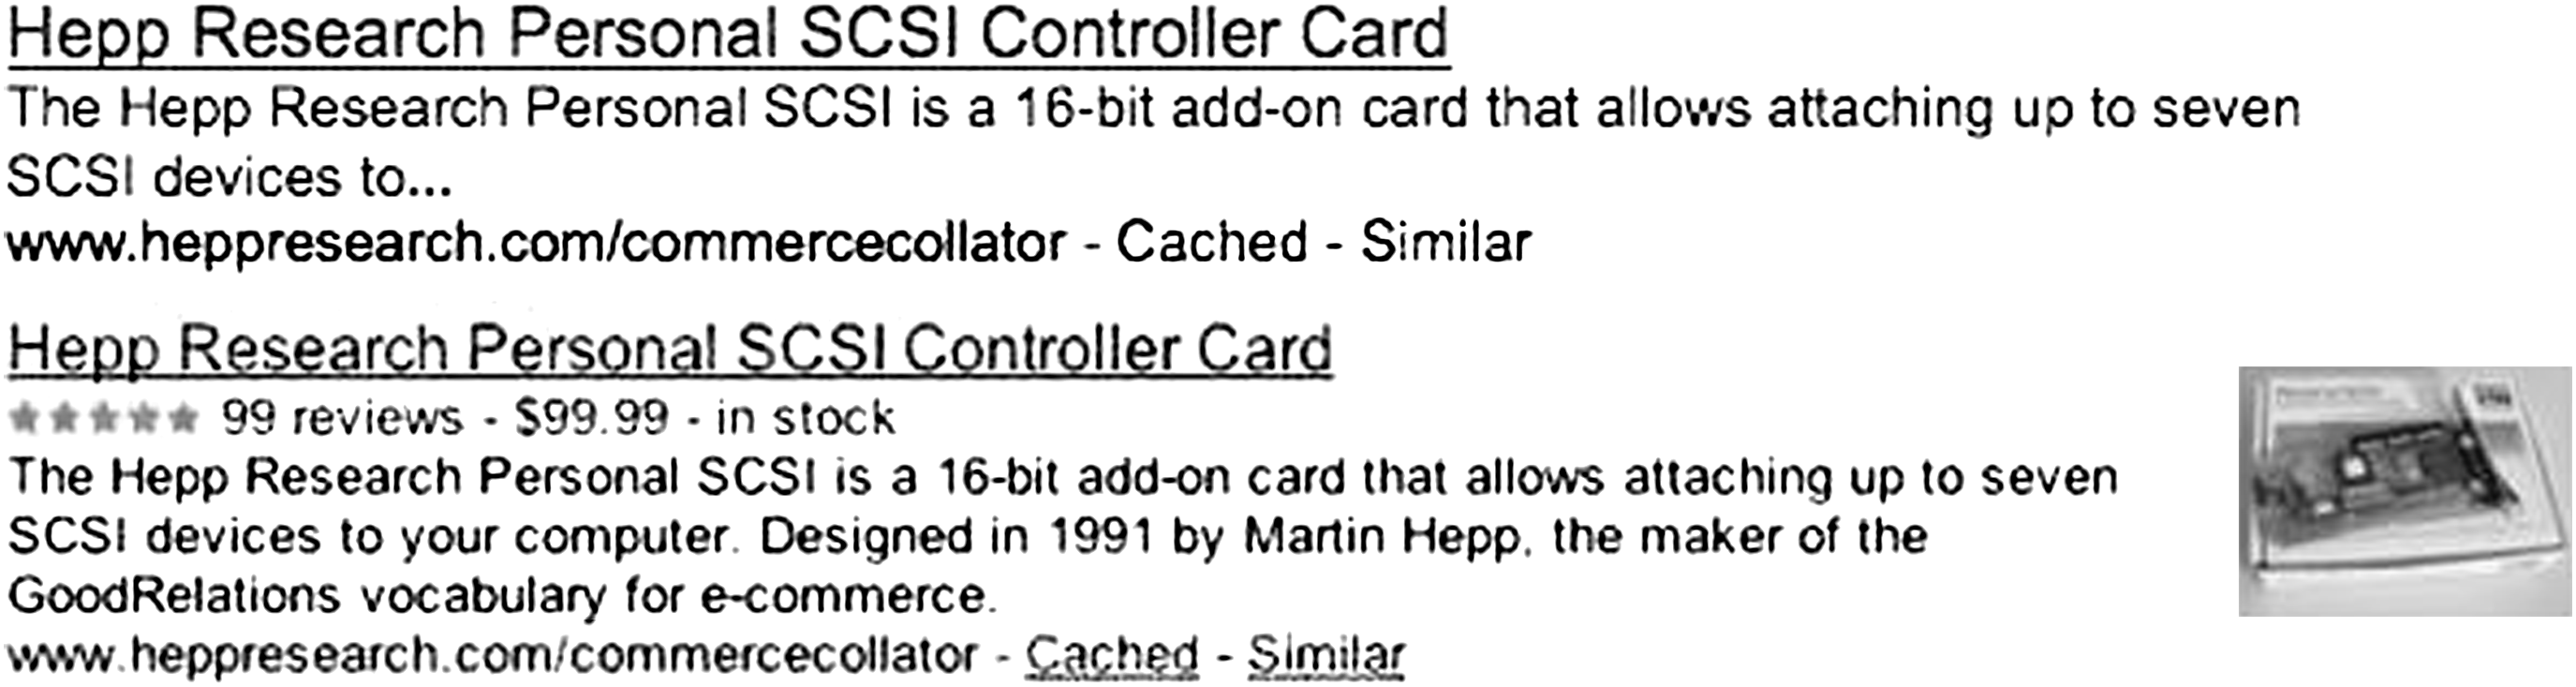
\includegraphics[width=5in]{media/ch14/f14-01.png}
\caption{Google search results for the same product, without (top) and with
(bottom) GR markup.}
\label{fig:ch14.01}
\end{figure}




GR provides a way to express that a company is making an offer of a
product or a service. This is expressed in three classes in GR:

\begin{lstlisting}
gr:BusinessEntity a owl:Class .
gr:Offering a owl:Class .
gr:ProductOrService a owl:Class .
gr:offers a owl:ObjectProperty ;
          rdfs:domain gr:BusinessEntity ;
	  rdfs:range gr:Offering .
gr:includes a owl:ObjectProperty ;
            rdfs:domain gr:Offering ;
	    rdfs:range gr:ProductOrService .
\end{lstlisting}

This provides the basic framework of how a business offering is
described in GR. GR provides many ways to enhance a description of an
offering, based on these three things. We'll illustrate how this works
with a real example of a business that uses GR and RDFa on its web site
to enhance Search Engine Optimization.

\begin{example}{Plush Beauty Bar}

The Plush Beauty Bar in West Hollywood has used RDFa to mark up its web
site,
\href{http://plushbeautybar.com/\%20}{{http://plushbeautybar.com/}},
using the Good Relations ontology. We will use their markup as an
example of the use of GR. The particular information in this example is
for educational purposes only, and does not correspond to any real
offerings by the Plush Beauty Bar. In this exposition, we will use the
namespace prefix plush: for all resources defined by Plush Beauty Bar.

The Plush description begins with the business entity itself, the
PlushBeautyBar. It offers several services,
including a basic manicure (shiny buff or polish):

\begin{lstlisting}
plush:Business a gr:BusinessEntity ;
               gr:offers plush:Offering_1 ;
	       gr:offers plush:Offering_2 ;
	       gr:offers plush:Offering_3 .
plush:Offering_1 rdfs:label "NAIL SERVICES (shiny buff or polish)" .
\end{lstlisting}

GR allows Plush to specify what kind of client they are advertising
to---is this a Business-to-Business shop or a Business-to-Consumer shop?
A nail salon is of course the latter---they are selling to individuals
who want to buy a service. GR includes a property called
gr:eligibleCustomerTypes for this. Its range is a class called
BusinessEntityType, that includes a handful of predefined business
entities that Plush can choose from:

\begin{lstlisting}
gr:eligibleCustomerType a owl:ObjectProperty ;
     rdfs:domain gr:Offering ;
     rdfs:range gr:BusinessEntityType .
gr:Business a gr:BusinessEntityType .
gr:Enduser a gr:BusinessEntityType .
gr:PublicInstitution a gr:BusinessEntityType .
gr:Reseller a gr:BusinessEntityType .
\end{lstlisting}

Plush expresses its desired end customer as a selection from these
business entity types:

\begin{lstlisting}
plush:Offering_1 gr:eligibleCustomerType gr:Enduser .
\end{lstlisting}

In a similar fashion, GR provides predefined classes of business
functions, payment methods, delivery methods, warranty scopes, etc.,
along with corresponding properties. Plus uses some of these to describe
its offering as well:

\begin{lstlisting}
plush:Offering_1
     gr:acceptedPaymentMethods
         gr:Cash , gr:Discover , gr:VISA , gr:MasterCard ;
     gr:hasBusinessFunction gr:ProvideService .
\end{lstlisting}

Plush's services come at a price, of course, and GR allows Plush to
describe these, as well. This poses a modeling problem---if we were to
define a property called, say, :cost, that related an offering to a
number, we could specify the amount of the price, but in business we
need to know more about the cost than just the number, we need to know
currency as well. This means that we have to put some more information
on the cost relationship between the offering and its price. This is an
example of reification from Chapter~\ref{ch3}, and GR solves it by defining a
class called a UnitPriceSpecification for the full description of a
price. We'll see how Plush uses this to describe the price of their
manicure:

\begin{lstlisting}
plush:Offering_1 gr:hasPriceSpecification plush:PriceSpec_1 .
plush:PriceSpec_1 a gr:UnitPriceSpecification ;
        gr:hasCurrency "USD"^^xsd:string ; 
	gr:hasCurrencyValue "19"^^xsd:float ; 
	gr:hasUnitOfMeasurement "C62" .
\end{lstlisting}

This says that the manicure offering has a price, which is \$19 (US).
The unit of measure is worth looking at, since units of measure play a
key role in commerce. GR uses the United Nations standard called UNECE
for referring to measurement units; ``C62'' is the unit for ``by the
job.'' If instead Plush were charging by the hour, the unit would be the
UNECE unit for hour, ``HUR.''

This offering is for a particular service; we have seen the price, the
methods of payment, the kinds of
customer, but we haven't yet talked about the service itself. An
offering can include several services, but in this case, the offering
includes just one---the basic manicure. This is stated simply as:

\begin{lstlisting}
plush:Offering_1 gr:includes plush:Service_1 .
plush:Service_1 a gr:ProductOrService ; 
        rdfs:label "NAIL SERVICES: Manicure" .
\end{lstlisting}

The information Plush expresses about its manicure offering is shown in
Figure~\ref{fig:ch14.02}

We can query this structure of this sort to answer questions like,
``Show me the services for individual customers (i.e., end users) that
cost less than \$20'' with SPARQL as follows:

\begin{lstlisting}
SELECT ?service
WHERE {?o a gr:Offering ;
          gr:eligibleCustomerTypes gr:EndUser ; 
          gr:includes ?s ;
          gr:hasPriceSpecification ?ps .
       ?ps gr:hasCurrencyValue ?v;
          gr:hasCurrency "USD" .
       ?s rdfs:label ?service .
       FILTER (?v < 20)
}
\end{lstlisting}


\begin{figure}
\centering
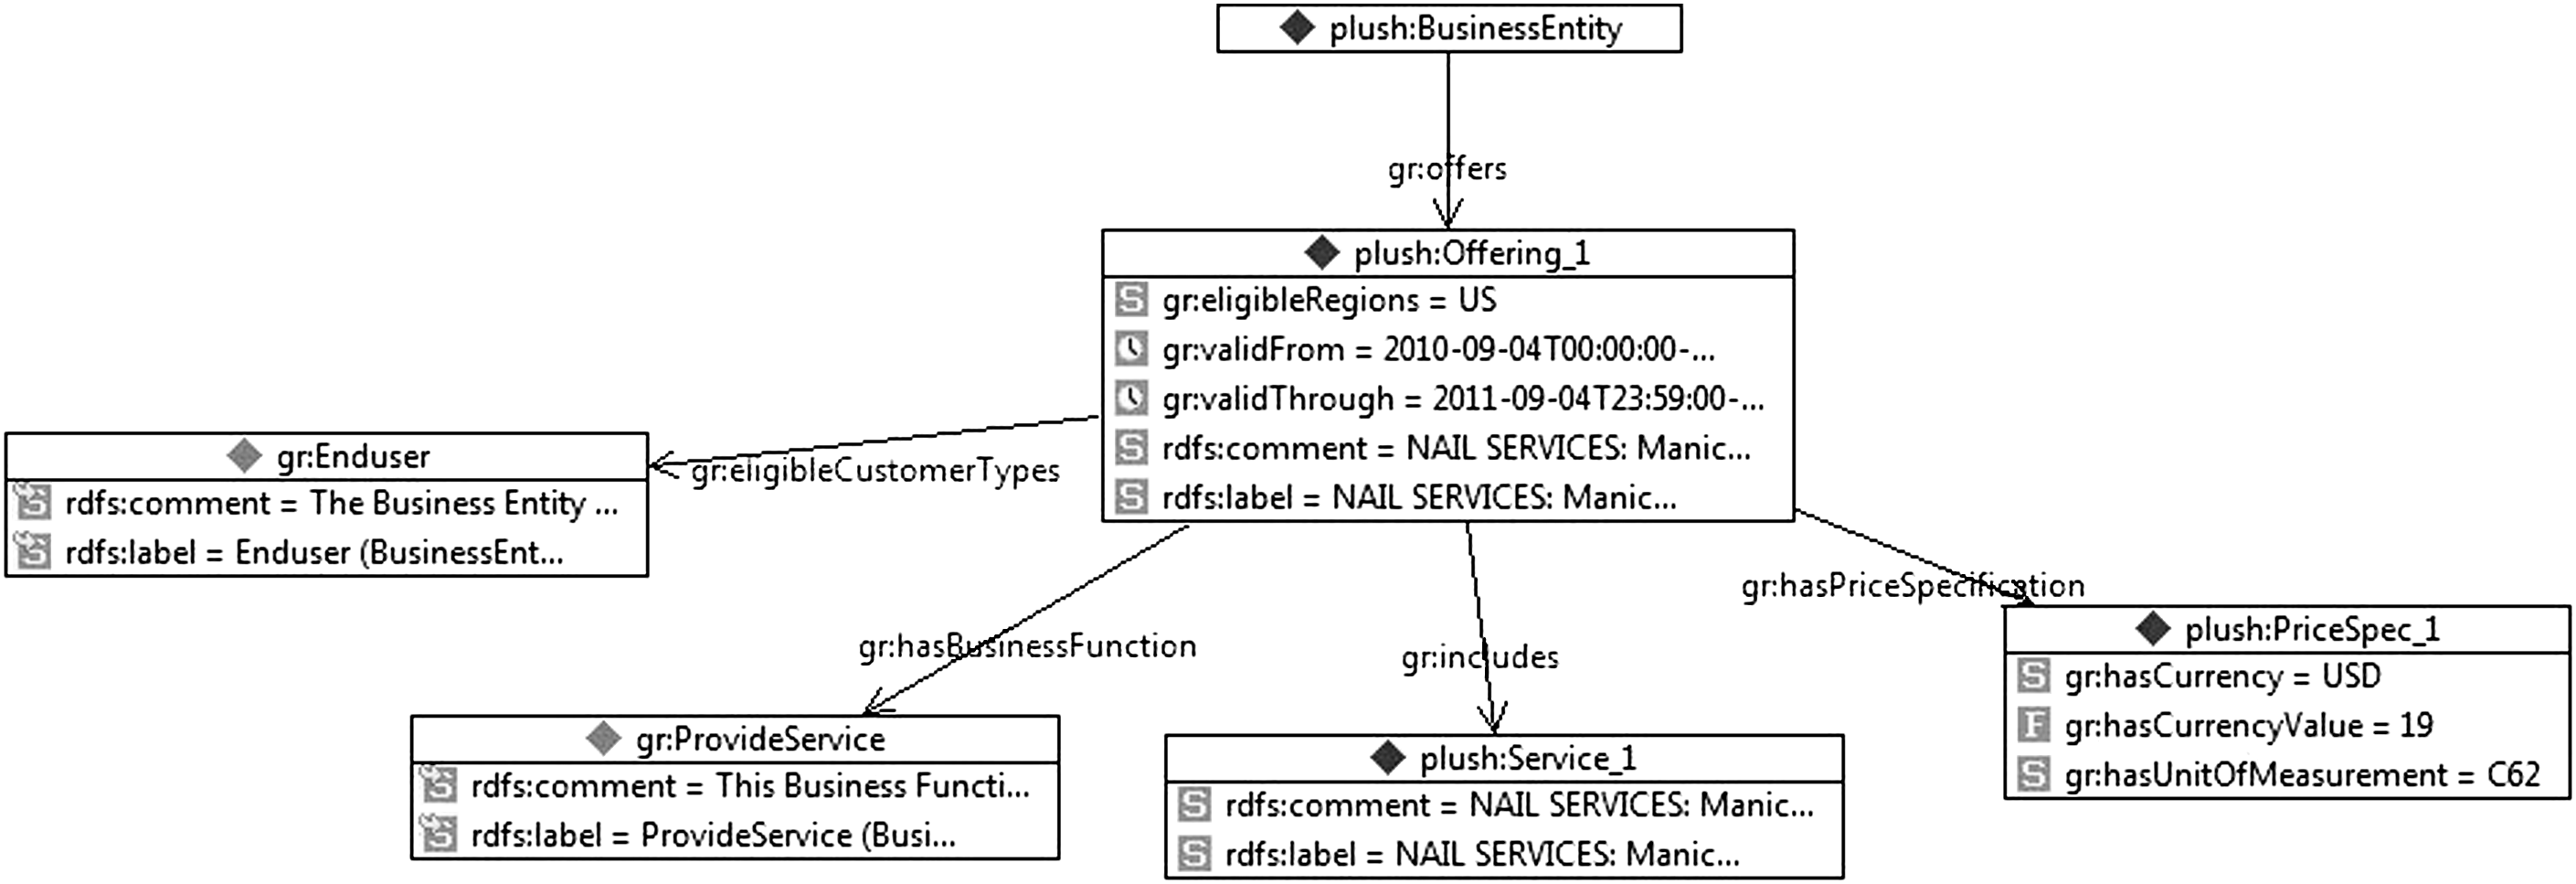
\includegraphics[width=5in]{media/ch14/f14-02.png}
\caption{Information about Plush's manicure offering, shown in graph form.}
\label{fig:ch14.02}
\end{figure}



The results will list all the services in that price range; a regular
search engine can filter those based on keywords, to focus on the
particular service desired.
\end{example}

\section{Inferencing in the Good Relations Ontology}

Suppose that in addition to its manicure services, Plush were to offer a
massage service, priced by the hour. If we wanted to describe a
one-and-a-half-hour massage session, the notion of includes would have
to be reified, just as we did for the price. GR provides a means to do
this, by introducing the notion of a \texttt{TypeAndQuantityNode}:

\begin{lstlisting}
plush:Offering_2 a gr:Offering ; 
     gr:includesObject plush:Quantity_2 .
plush:Quantity_2 a gr:TypeAndQuantityNode ; 
     gr:typeOfGood plush:Service_2 ; 
     gr:hasUnitOfMeasurement "HUR" ; 
     gr:amountOfThisGood "1.5"^^xsd:float .
plush:Service_2 a gr:ProductOrService ;
     rdfs:label "Relaxing Massage" .
\end{lstlisting}

This model differs from the description of the manicure in two ways;
first, it includes the intermediate entity \texttt{Quantity\_1} that allows us
to make multiple statements about the massage service; in particular,
that it lasts for 1.5 hours. The second difference is that the property
used to connect the offering to the (reified) service description is
includesObject (whereas it was includes in the manicure example). This
is how GR indicates the reified relationship, by using the property
\texttt{includesObject} to indicate the service.

This method for representing services by the hour (or any other good
that is sold in some units) is
expressive and consistent, but it does pose a problem when it comes to
querying a Good Relations data
set. If we represent massages as we have done here, and manicures as we
did in the previous example, we can't query both structures using just
the query we used for manicures---we will need a query that knows how to
work with both ways of representing services.

One solution to this would be to retire the simple representation of
services---the one that uses the predicate \texttt{includes},  we used for
the manicure---in favor of the more expressive representation using
includesObject. This is certainly possible---we could represent the
manicure as being a service, measured ``by the job,'' i.e., unit
``C62,'' where the amount is 1. Then the manicure representation would
look like

\begin{lstlisting}
plush:Offering_1 a gr:Offering ;
    gr:includesObject plush:Quantity_1 .
plush:Quantity_1 a gr:TypeAndQuantityNode ;
    gr:typeOfGood plush:Service_1 ;
    gr:hasUnitOfMeasurement "C62" ;
    gr:amountOfThisGood  "1" .
plush:Service_1 a gr:ProductOrService ;
    rdfs:label "NAIL SERVICES: Manicure " .
\end{lstlisting}

But this is a lot of work to go through, in comparison to the much
simpler representation we are already using, i.e.,

\begin{lstlisting}
plush:Offering_1 gr:includes plus:Service_1 .
\end{lstlisting}

Do we really have to abandon this simple representation, and go for the
more complex one? Good Relations includes a number of ``Optional
Axioms''---these are rules that apply to the
Good Relations ontology, but are not expressed in the OWL representation
of Good Relations. They are described on the Good Relations web site
both in plain English, as well as in SPARQL.\footnote{http://www.ebusiness-unibw.org/wiki/GoodRelationsOptionalAxiomsAndLinks} One of these rules is
designed exactly for this case. A simplified version of the rule can be
expressed in SPARQL as

\begin{lstlisting}
CONSTRUCT {
?o gr:includesObject _:n .
_:n rdf:type gr:TypeAndQuantityNode.
_:n gr:amountOfThisGood "1.0"^^xsd:float .
_:n gr:hasUnitOfMeasurement "C62"^^xsd:string.
_:n gr:typeOfGood ?p. }
WHERE
{
?o rdf:type gr:Offering .
?o gr:includes ?p . 
}
\end{lstlisting}

That is, if an offering gr:includes something, then construct a
\texttt{TypeAndQuantityNode} with units ``C62'' (``by the job'') and amount
1 --- building in the reified structure. Figure~\ref{ch114.03} shows the result of
constructing these triples for the manicure example.



\begin{figure}
\centering
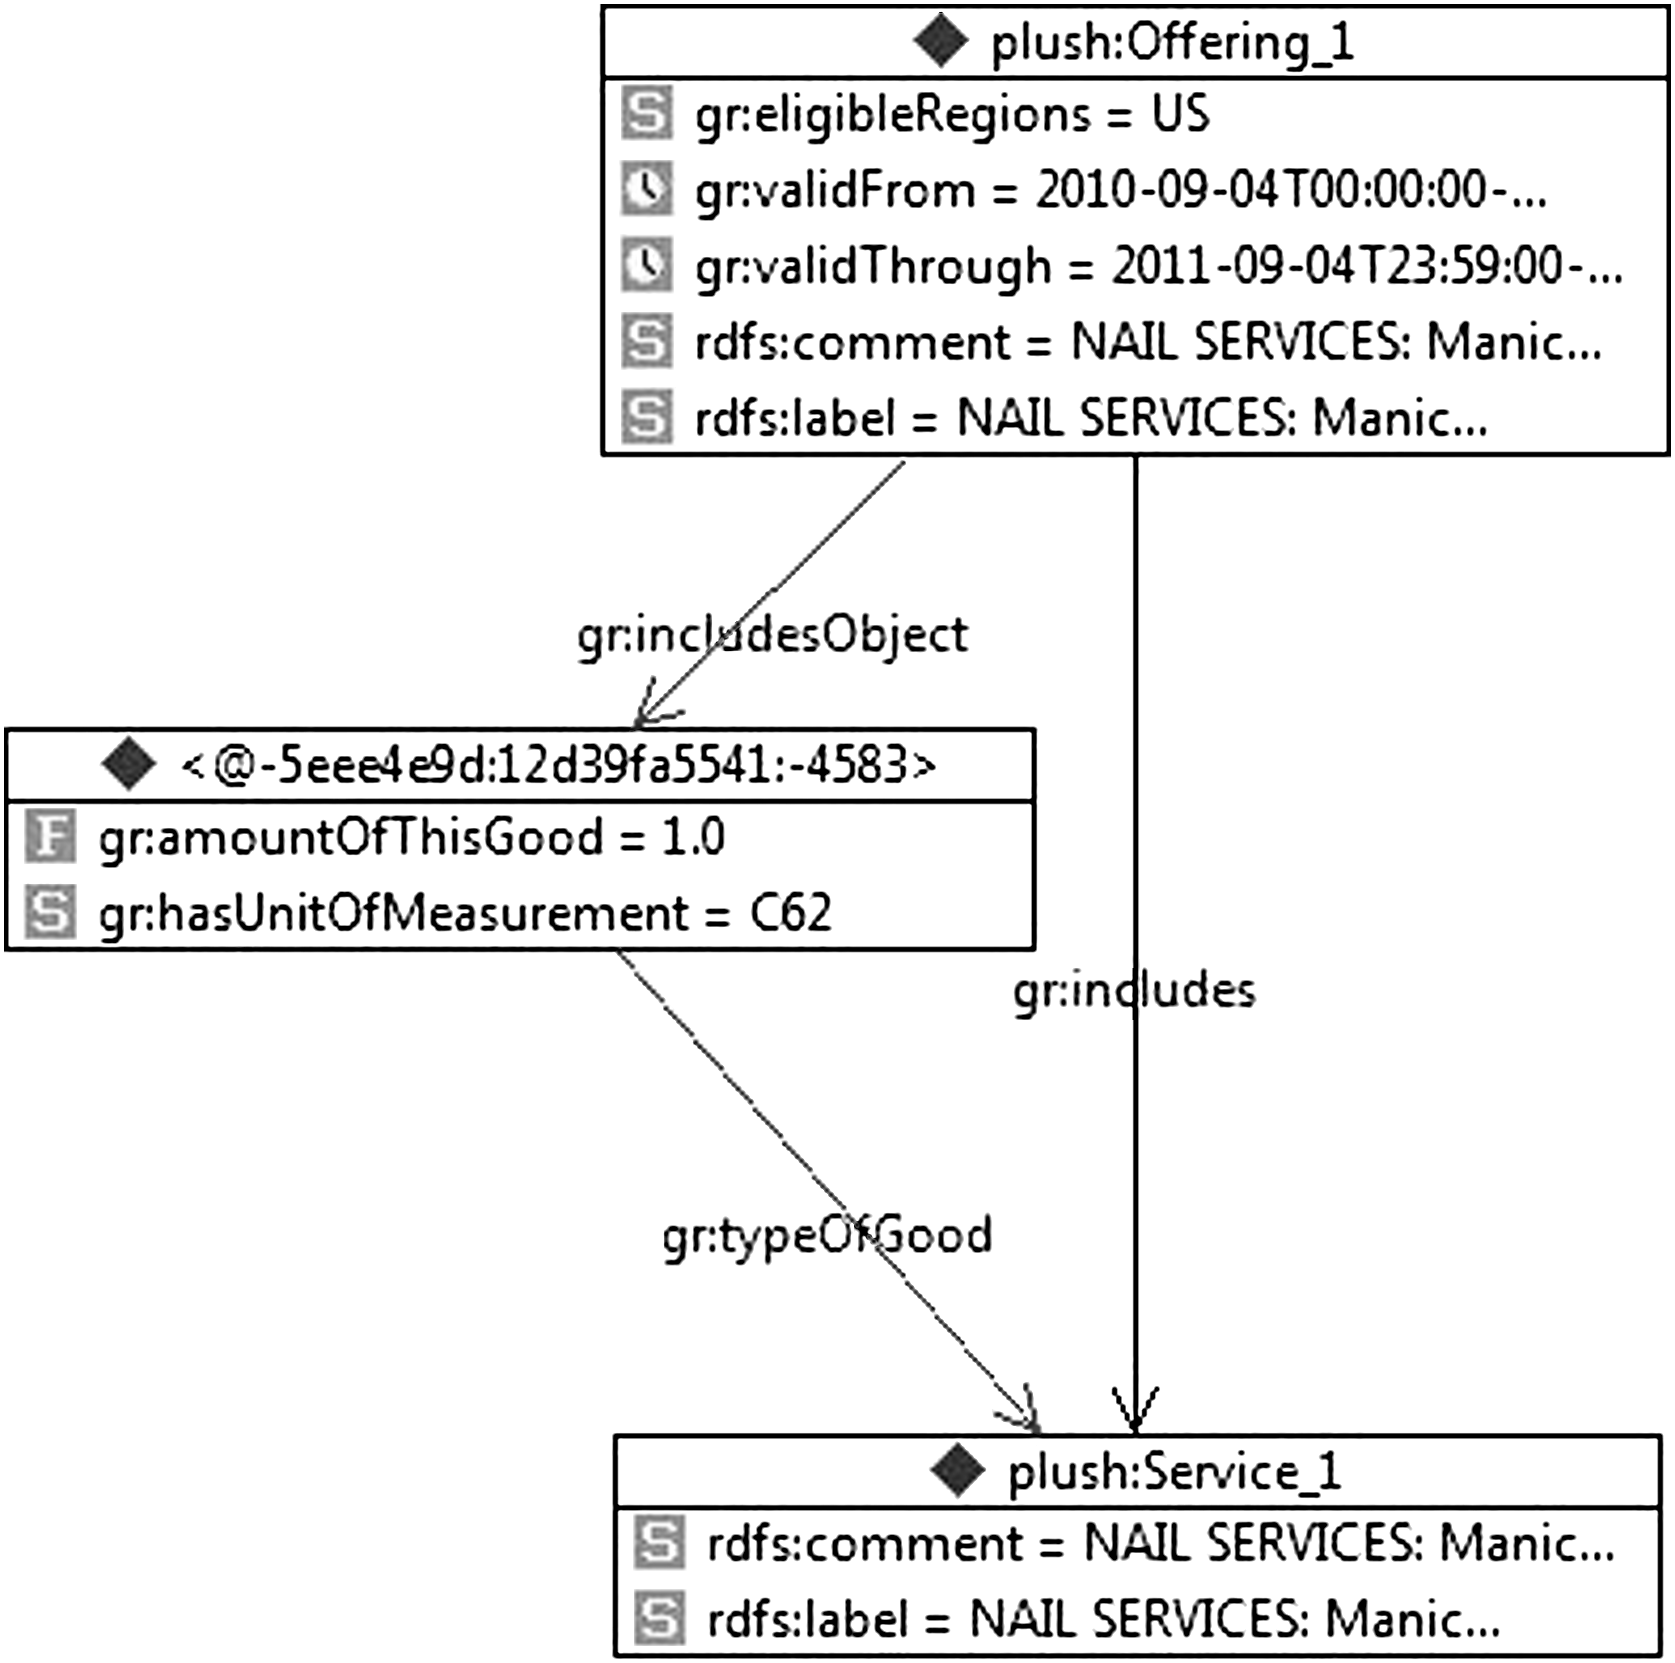
\includegraphics[width=5in]{media/ch14/f14-03.eps}
\caption{Offering\_1 after inferencing; the reified object has been constructed
from the asserted includes triple.
}
\label{fig:ch14.03}
\end{figure}




\section{Composing Files}

The Optional Axioms of Good Relations are not represented as part of the
published GR ontology. The reason for this is that most of the optional
axioms cannot be expressed in OWL, and the GR authors want GR to be an
OWL ontology. But these rules can be expressed in languages that go
beyond OWL. We want to leave the published GR ontology ``pure'' OWL,
while having the non-OWL parts in another file. Most software languages
have features for managing modularity of this sort, and OWL is no
exception; it has language features for modularizing semantic models.
These language features have no semantics for the model (they allow no
new triples to be inferred), but they help us, as humans, to organize a
model in a modular way.

\subsubsection{owl:Ontology}

OWL provides a built-in class whose members correspond to modular parts
of a semantic model. It is customary for the URI of an Ontology to
correspond to the URL of the file on the Web where the ontology is
stored. This makes use of a slightly different syntax in Turtle than we
have used so far. It is possible to spell out a URI by enclosing it in
angle brackets:

\begin{lstlisting}
<http://www.workingontologist.com/Examples/ch14/shakespeare.owl>
        a owl:Ontology.
\end{lstlisting}

Unlike the other constructs in OWL, the meaning of membership in
\texttt{owl:Ontology} is not given by inference. In fact, one could say that it
has no formal meaning at all. Informally, a member of \texttt{owl:Ontology}
corresponds to a set of RDF triples. The set of triples such a resource
corresponds to can be found by de-referencing its URI (as a URL), which
is expected (informally) to resolve to an RDF data set (e.g., an RDF
file). Formally, there is no connection in the model between an instance
of \texttt{owl:Ontology} and the triples to which it corresponds.

Although such an individual has no significance from the point of view
of model semantics, it can
be quite useful when specifying modularity of semantic models. The
primary way to specify modularity is with the property \texttt{owl:imports}.

\subsubsection{owl:imports}

This is a property that connects two instances of the class
\texttt{owl:Ontology}. Just as is the case with \texttt{owl:Ontology} itself, no
inferences are drawn based on \texttt{owl:imports}. But the meaning in terms of
modularity of models is clear: When any system loads triples from the
file corresponding to an instance of \texttt{owl:Ontology}, it can also find any
file corresponding to an imported ontology and load that as well. This
load can, in turn, trigger further imports, which trigger further loads,
and so on. There is no need to worry about the situation in which there
is a circuit of imports (e.g., GR imports OGP imports FOAF imports GR).
A simple policy of taking no action when a file is imported for a second
time will guarantee that no vicious loops will occur. The resulting set
of triples is the union of all triples in all imported files.

In the case of GR, we can separate its rules out into a separate file,
and have that file import the GR ontology. If someone just wants the
``pure OWL'' GR ontology, they can import it from its base URI,
http://purl.org/goodrelations/v1.
If someone else wants the GR ontology together with its (non-OWL) rules,
they can import
http://WorkingOntologist.org/Examples/Chapter13/GROptionalAxioms,
which expresses these rules in a non-OWL rules language called SPIN,
found at spinrdf.org.

\begin{lstlisting}
<http://WorkingOntologist.org/Examples/Chapter13/GROptional_Axioms>
       rdf:type owl:Ontology ;
       owl:imports <http://purl.org/goodrelations/v1> ;
       owl:imports <http://spinrdf.org/spin> ,
\end{lstlisting}

SPIN is a very simple, SPARQL-based rules language that works by linking
classes in an ontology to SPARQL CONSTRUCT queries. To express one of
the optional axioms in SPIN, we simply assert a triple that relates a
query to the relevant class. The axiom we saw in the previous section
applied to offerings, so we associate the query that defines the rule
with the \texttt{gr:Offering} class as follows:

\begin{lstlisting}
gr:Offering spin:rule
"CONSTRUCT {
 ?o gr:includesObject _:n .
 _:n rdf:type gr:TypeAndQuantityNode .
 _:n gr:amountOfThisGood "1.0"^^xsd:float .
 _:n gr:hasUnitOfMeasurement "C62"^^xsd:string .
 _:n gr:typeOfGood ?p . }
 WHERE
 {
 ?o rdf:type gr:Offering .
 ?o gr:includes ?p. }"
\end{lstlisting}

In this example, we have represented the query associated with
\texttt{gr:Offering} as a string; SPIN also includes a way to represent the query
in RDF that is often more convenient for storage, but is not as
convenient for reading in a book. Associating a rule (in the form of a
CONSTRUCT query) with a class allows us to specify the scope of each of
the rules, and to express them in a familiar language. Like Good
Relations itself, there is a lot more to SPIN, and the interested reader
is referred to http://spinrdf.org/.

\subsection{Summary}

The Good Relations ontology provides a way in which Web content
providers can mark up their web pages to describe business offerings.
Like OGP, its designers have made a commitment to simplicity. But as GR
is more ambitious than OGP, it provides a good deal more sophistication
in the model for providing structured descriptions of goods and
services. GR both provides standards of reference for describing
business entities (like \texttt{gr:EndUser} and \texttt{gr:ProvideService}), as well as
referring to other standards (like the UN/CEFACT codes for units of
measure). As such, it is a good Semantic Web citizen, providing linkages
to familiar vocabularies as well as contributing its own.

To date, Good Relations has been used for Search Engine Optimization,
with considerable impact. But the real value to having structured data
is to support true semantic search, whereby a customer can be very
specific about what they are searching for, and have some confidence
that if it exists, then it can be found. Good Relations has made great
strides in this direction, by achieving structured markup in tens of
thousands of sites.

\section{Quantities, Units, and Dimensions}
\label{QUDT}

As part of the Constellation Program, NASA developed an ontology to deal
with units of measure. The utility of controlling references to units in
science and engineering has been understood for centuries, and there are
several standard systems of units; there is the US Customary set of
units (with things like miles, feet, and degrees Fahrenheit), the
international system (``SI'') that includes meters, kilograms, and
Kelvins. NASA built an ontology of Quantities, Units, and Dimensions
(QUDT)\footnote{QUDT also includes information about Types, which is beyond the scope
of this treatment.}
to capture and manage this information.

What is the purpose of such an ontology? In contrast to OGP and Good
Relations, which provide vocabularies that assist web page developers in
marking up their pages, QUDT cuts across many domains. It was designed
for science and engineering, but it has applicability in any setting
where information can be expressed in different units. We have already
seen an application for units in the Good Relations ontology---it is
important to know how a service is measured---by the hour, by the
minute, or by the job.

QUDT serves three major purposes in the Semantic Web. First, it provides
a global reference for units. If one information source says that some
product is measured in pounds, and another source
says that its service is provided in pounds, how do we know that they
are making reference to the same notion of pound (there is more than
one)? QUDT provides a URI for the notion of pound (with information to
distinguish it from other units with the same common name), so that such
references can be made unambiguously. QUDT is not alone in providing
this service; as we have already seen with Good Relations, UN/CEFACT
also provides a canonical set of codes for unambiguously identifying
units. QUDT connects to the UN/CEFACT codes with the property
\texttt{qudt:uneceCommonCode}.

The second purpose that QUDT serves is to provide conversion services.
If two information sources
provide information in terms of pounds, and we use something like
UN/CEFACT or QUDT to determine that they are the same notion of pound,
then we can compare the offerings. But what if one of them offers a
product measured in pounds, and the other in kilograms? There are a few
things that have to happen before we can compare the offerings. First,
we have to understand whether it is even possible to compare pounds and
kilograms (are they ``commensurate'' values). If they are, then we need
to convert values from one unit to the other. QUDT offers both of these
services. These services are useful in science and engineering settings,
but also in more common settings like the commercial applications of
Good Relations.

The third purpose that QUDT serves is mostly focused on engineering
settings, where it is often important to verify the dimensions of
certain quantities. One way to check for errors in a formula is to check
the dimensions of the components of a formula; only quantities with the
same dimensions may be added to one another or compared to one another;
for example, it makes no sense to add kilograms and centimeters or to
compare seconds to feet. A simple check for correct dimensions can turn
up errors, even in quite complex formulas. QUDT includes a comprehensive
model of dimensions, cross- referenced with units, which enables
dimension-based calculations. The simplest application of this facility
is for units conversion---it makes no sense to convert from one unit to
another, if the units don't have the same dimension. The formula to
convert from meters to feet, 1m = 3.28 ft, can be checked for
dimensional correctness---do meters and feet have the same dimension?
Yes, they do; both are measures of length.

We will explore just enough of the QUDT ontology to show how it supports
these three functions. The QUDT ontology supports this functionality
through a careful separation of Quantities, Units, and Dimensions. In
some sense, there is nothing new about this separation; treatment of
these things has been ongoing in science and engineering for centuries.
QUDT makes it referenceable on the Web and actionable. Further
information about QUDT can be found at its web site, QUDT.org.

A \emph{Quantity} is some measurable property. A \emph{Quantity Kind} is,
appropriately enough, the kind of thing one can measure---familiar
quantity kinds are length, time, mass, and force, etc. A \emph{Unit} is a
standard of measurement for a particular quantity kind. A foot is a unit
for measuring length; a second is a unit for measuring time. It is
common to have several units for a single kind; feet, inches,
kilometers, Angstroms, light-years, and furlongs are all measures for
length.

QUDT uses the \emph{Local Restriction of Range} pattern described in Chapter\ref{ch12}; that is, it uses
\texttt{owl:allValuesFrom} to restrict the possible values for a property. The
relationship between \texttt{qudt:Unit} and \texttt{qudt:QuantityKind} is called
\texttt{qudt:quantityKind} (note the naming convention; \texttt{qudt:quantityKind} begins
with a lower-case letter, and hence is a property; \texttt{qudt:QuantityKind}
begins with an upper-case letter and is a class). The restriction on
this relationship is defined as

\begin{lstlisting}
qudt:Unit a owl:Class ;
   rdfs:subClassOf
       [ a owl:Restriction ;
         owl:allValuesFrom qudt:QuantityKind ;
         owl:onProperty qudt:quantityKind
       ] .
qudt:quantityKind a owl:ObjectProperty .
qudt:QuantityKind a owl:Class .
\end{lstlisting}


As an example of units and quantity, let's have a look at feet and
length:

\begin{lstlisting}
vocab-units:Foot a qudt:Unit ;
      qudt:quantityKind vocab-quantities:Length .
\end{lstlisting}

Following along as in the example of this pattern from Chapter 12, from
these triples we can infer that

\begin{lstlisting}
vocab-quantities:Length a qudt:QuantityKind .
\end{lstlisting}

QUDT includes a comprehensive list of units and quantities from many
fields of science, including mechanics, thermodynamics, chemistry,
informatics, and biology. It organizes its namespaces in a modular
way---as we saw in this example, resources that describe how units work
(like the resources \texttt{qudt:QuantityKind} and \texttt{qudt:Unit}) are in the qudt:
namespace, while particular quantities and units (like
vocab-\texttt{quantities:Length} and vocab-\texttt{units:Foot}) are in namespaces whose
names begin with vocab-. These resources are so named because together
they form controlled vocabularies; one for quantities and one for units.
These resources resolve the first function of the QUDT vocabulary, that
is, they provide unambiguous reference URIs for all the units and
quantities in QUDT.

\subsection{Converting Units with QUDT}

QUDT includes information that can be used to convert measurements from
one unit to another. This is a workhorse for merging quantitative
information on the Semantic Web. Conversions can be within the same
system of units (meters to kilometers, seconds to hours, feet to miles)
or crossing between systems (miles to kilometers, degrees Fahrenheit to
degrees Centigrade). In order for such a conversion to make sense, the
units must be commensurate---that is, they measure the same kind of
thing. Miles and kilometers are both measurements of length, so it makes
sense to consider a conversion between the two. Seconds and degrees
Fahrenheit do not measure the same thing; it is not meaningful to
convert from one to another.

Usually we can tell if two units are commensurate if they measure the
same quantity kind, but in some cases, certain different quantity kinds
are in fact commensurate. These are important situations, in that they
usually reflect a deep connection between different scientific domains.
For example, the law of Conservation of Energy states that energy is
preserved in an interaction---but energy can take many forms, including
thermal energy (heat), potential energy, kinetic energy, and others.
Measurements of all these kinds are commensurate. QUDT represents this
situation with a tree structure using a property called
\texttt{qudt:generalization}. In particular,

\begin{lstlisting}
vocab-quantities:KineticEnergy qudt:generalization vocab-quantities:EnergyAndWork .
vocab-quantities:PotentialEnergy qudt:generalization vocab-quantities:EnergyAndWork .
vocab-quantities:ThermalEnergy qudt:generalization vocab-quantities:EnergyAndWork .
\end{lstlisting}

This means that we can query for whether two units are commensurate with
the following SPARQL
query:

\begin{lstlisting}
ASK WHERE {
?arg1 qudt:quantityKind ?kind1 .
?arg2 qudt:quantityKind ?kind2 .
?kind1 qudt:generalization* ?kind .
?kind2 qudt:generalization* ?kind .
\end{lstlisting}

That is, \texttt{?arg1} and \texttt{?arg2} are commensurate, if their associated quantity
kinds are related to a common ancestor in the \texttt{qudt:generalization} tree.
Recall that \texttt{qudt:generalization}* will match zero or more repeated
occurrences of \texttt{qudt:generalization}, so that if \texttt{?kind1} and \texttt{?kind2} are the
same thing (e.g,. Length), they will match; this means that the query
will return true for \texttt{?arg1} bound to \texttt{vocab-units:Foot} and \texttt{?arg2} bound to
\texttt{vocab-units:Meters}. It will also return true for
\texttt{vocab-quantities:PotentialEnergy} and \texttt{vocab-quantities:ThermalEnergy},
because they both have a common generalization,
\texttt{vocab-quantities:EnergyAndWork}.

Once we have determined that two units are commensurate, we can set
about converting measurements in one unit to the other. Each unit
includes two properties---\texttt{qudt:conversionMultiplier} and
\texttt{qudt:conversionOffset}. As their names suggest, these provide conversion
multipliers and offsets for each unit. For each dimension, there is a
base unit for which the multiplier is 1 and the offset 0. It isn't
important to know what the base unit is, in order to convert from one
unit to the other. For example, to convert ten kilometers to miles, we
can use the query

\begin{lstlisting}
SELECT (((((10.0 * ?M1) + ?O1) - ?O2) / ?M2) AS ?value)
WHERE {
    unit:Kilometer qudt:conversionMultiplier ?M1 ;
    qudt:conversionOffset ?O1 .
    unit:MileInternational qudt:conversionMultiplier ?M2 ;
    qudt:conversionOffset ?O2 .
}
\end{lstlisting}

Answer: \textbf{6.2137119223733395}

QUDT includes over five hundred conversion factors, enabling thousands
of such conversions.

\subsection{Using QUDT conversions}

We can express these conversions in a SPARQL query, but this isn't
available as an inference. That is, if we have some quantity specified
in miles, we can't always count on an inference engine to express that
value in kilometers. Calculations of this sort are the sort of things
that one usually puts into an application program. SPIN is an example of
how to do this. SPIN is a proposal for a way to work with SPARQL in a
programmatic way. Earlier in Chapter~\ref{ch7} we saw how SPIN could be used to
attach queries to an ontology. Here we see another application of SPIN.
The query we used to convert kilometers to miles required us to put the
information about the conversion into the query; the number to be
converted (10.0), the source unit (kilometer), and the target unit
(mile). If we want to do another conversion, we would need another
query, very similar in form, but with a different measurement and
different designations of units. Far more convenient would be to
parameterize the query, making it effectively into a function
definition. The generalized query, using variables ?arg1, ?arg2, etc.,
for the function arguments, looks like

\begin{lstlisting}
SELECT (((((?arg1 * ?M1) + ?O1) - ?O2) / ?M2) AS ?value)
WHERE {
    ?arg2 qudt:conversionMultiplier ?M1 ;
    qudt:conversionOffset ?O1 .
    ?arg3 qudt:conversionMultiplier ?M2 ;
    qudt:conversionOffset ?O2 .
}
\end{lstlisting}

SPIN allows such queries to be given names, which themselves are
resources in RDF. If we give this query the name \texttt{qudtspin:convert}, then
we could write the 10 kilometer query simply as

\begin{lstlisting}
SELECT (qudtspin:convert(10.0, unit:Kilometer, unit:MileInternational)
                   AS ?value)
WHERE {}
\end{lstlisting}

The function call to \texttt{qudtspin:convert} is doing all the work---there is
nothing in the
WHERE clause to match at all!

The conversion of 32 degrees Fahrenheit to Centigrade looks very
similar:

\begin{lstlisting}
SELECT (qudtspin:convert(32.0, unit:DegreeFahrenheit,
unit:DegreeCelsius)
AS ?value)
WHERE {}
\end{lstlisting}

Answer: 0.0

\begin{challenge}{Comparison Shopping with Good Relations}
\label{chal:38}

Now that we can use QUDT to convert values from one unit to another, wec
an apply this to Good Relations data for purposes of comparison
shopping.

At the end of the Good Relations section, we had an example of a massage
service. Let's add some pricing information to it---a single
one-and-a-half-hour session costs US\$80.00.

\begin{lstlisting}
plush:Offering_2 a gr:Offering ;
    gr:hasPriceSpecification plush:PriceSpec_2 ;
    gr:includesObject plush:Quantity_2 .
plush:Quantity_2 a gr:TypeAndQuantityNode ;
    gr:typeOfGood plush:Service_2 ;
    gr:hasUnitOfMeasurement "HUR" ;
    gr:amountOfThisGood "1.5"^^xsd:float .
plush:Service_2 a gr:ProductOrService ;
    rdfs:label "Relaxing Massage" .
plush:PriceSpec_2 a gr:UnitPriceSpecification ;
    gr:hasCurrency "USD"^^xsd:string ; 
   gr:hasCurrencyValue "80.00"^^xsd:float .
\end{lstlisting}

Down the street from Plush, a competing day spa has its own offer---a
fifteen-minute chair massage, for the busy person-on-the-go:

\begin{lstlisting}
dayspa:Offering_3 a gr:Offering ;
          gr:hasPriceSpecification
          dayspa:PriceSpec_3 ;
	  gr:includesObject dayspa:Quantity_3 .
dayspa:Quantity_3 a gr:TypeAndQuantityNode ;
          gr:typeOfGood dayspa:Service_3 ;
	  gr:hasUnitOfMeasurement "MIN"^^xsd:string ;
	  gr:amountOfThisGood "15"^^xsd:float .
dayspa:Service_3 a gr:ProductOrService ;
rdfs:label "Chair Massage" . dayspa:PriceSpec_3 a
gr:UnitPriceSpecification ;
gr:hasCurrency "USD"^{}^{}xsd:string ;
gr:hasCurrencyValue "15.00"^{}^{}xsd:float .
\end{lstlisting}

Suppose we want to compare these two offerings in terms of their price
per minute of services. All the information is there---one of them costs
\$15 for 15 minutes, the other is \$80 for an hour and a half. But to
make the comparison, we have to convert the amounts into the same units.

We can do this by combining Good Relations with QUDT. First, we want to
query the Good Relations data to find out all the things we need to know
to make the comparison. We can do this simply by generalizing the common
data form into a query:

\begin{lstlisting}
SELECT *
WHERE {
?offering a gr:Offering ;
   gr:hasPriceSpecification ?pricespec ;
   gr:includesObject ?quantity .
?quantity a gr:TypeAndQuantityNode ;
   gr:typeOfGood ?service ;
   gr:hasUnitOfMeasurement ?UNunit ;
   gr:amountOfThisGood ?amt .
?service a gr:ProductOrService ;
   rdfs:label ?servicename .
   ?pricespec a gr:UnitPriceSpecification ;
   gr:hasCurrency ?currency ;
   gr:hasCurrencyValue ?price .
}
\end{lstlisting}

The graph pattern (the part after the keyword WHERE) corresponds line
per line to the data, with all the values that the two examples don't
have in common turned into variables. We have chosen names for the
variables that indicate their role in the graph; for example, \texttt{?pricespec}
is a \texttt{UnitPriceSpecification}; \texttt{?UNunit} is the designator for the units,
using the United Nations UNECE standard (as is common practice with Good
Relations).

We want to be able to use the conversion capabilities of QUDT on this
information, so we need to link our Good Relations results to QUDT. The
linkage point is, of course, the units. But Good Relations doesn't
reference QUDT units directly---it references UNECE units. Fortunately,
QUDT also references the UNECE units, with a property called
\texttt{qudt:uneceCommonCode}. We can get the QUDT units by matching a triple
using this property:

\begin{lstlisting}
?qudtunit qudt:uneceCommonCode ?UNunit .
\end{lstlisting}

Now we are in a position to compute a comparable cost rate in price per
minute. The choice of ``minutes'' here is somewhat arbitrary---we could
have as easily chosen any other time unit, like seconds or hours. Now
that we know what units (?qudtunit) the amount (?amt) is in, we can
convert it to minutes using \texttt{qudtspin:convert}:

\begin{lstlisting}
qudtspin:convert (?amt, ?qudtunit, unit:MinuteTime)
\end{lstlisting}

We can compute the cost per minute by dividing ?price by this. The final
query is

\begin{lstlisting}
SELECT ?servicename ?currency
       ((?price/qudtspin:convert(?amt, ?qudtunit,
                                 unit:MinuteTime))AS ?cost_per_min )
WHERE {
?offering a gr:Offering ;
    gr:hasPriceSpecification ?pricespec;
    gr:includesObject ?quantity .
?quantity a gr:TypeAndQuantityNode ;
    gr:typeOfGood ?service ;
    gr:hasUnitOfMeasurement ?UNunit ;
    gr:amountOfThisGood ?amt .
?service a gr:ProductOrService ;
    rdfs:label ?servicename .
    ?pricespec a gr:UnitPriceSpecification ;
    gr:hasCurrency ?currency ;
    gr:hasCurrencyValue ?price .
?qudtunit qudt:uneceCommonCode ?UNunit .
    }
ORDER BY ( ?cost_per_min )
\end{lstlisting}

Answer:

\begin{tabular}{|ll|}
\hline
servicename&currencycost\_per\_min\\
\hline
Relaxing Massage&USD 0.88\\
Chair Massage&USD 1.0\\
\hline
\end{tabular}

We have given the quotient of price per minute the name \texttt{?cost\_per\_min},
and sorted from lowest cost to highest. The result shows that the
Relaxing Massage is the better value per minute.
\end{challenge}

This example shows a number of features of the role that models play in
linking data sources. The structure of the Good Relations ontology gave
us a consistent way to represent offerings, prices, amounts, and units
of competing businesses. QUDT provides useful services (units
conversions) for computations over these data. But as often happens in
the data wilderness, these two models were not designed to connect. In
particular, the Good Relations model does not use QUDT as its
unambiguous reference for units. Fortunately, there is a common
reference shared by QUDT and Good Relations---namely, the United Nations
UNECE unit names standard. Since they both share a reference to UNECE,
the connection can be made (with a single triple in the graph pattern!).
The result is a price comparison based on published information, from a
single query over the combined data sets.

\subsection{DIMENSION CHECKING IN QUDT}

There are a lot of services that an engineer or scientist could ask of a
system of units; many of these go by the name dimensional analysis.
Whole books have been written on the subject; we can barely scratch the
surface of this topic here (therefore, see the Further Reading section
at the conclusion of the book). We will illustrate enough of the QUDT
ontology to show how it can support certain basic operations in
dimensional analysis.

The basic idea of dimensional analysis is that a quantity has a
signature that tells how it relates to
basic quantities like length, time, and mass. QUDT defines eight base
quantities of this sort, but in this exposition, we will focus on these
three. A compound quantity has a signature in these basic quantities.
For example, the compound quantity velocity is defined as a ratio
between distance and time; this means that its signature in terms of
length, time, and mass is length/time. The signature can be written as a
vector, with one vector component for each base unit, and the magnitude
of the vector in that component being the exponent of the base quantity
in the formula for the compound quantity. If we write our vectors in the
order {[}length, mass, time{]} then the vector for velocity is {[}1, 0,
-1{]}. The vector for any base quantity will have magnitude 1 in exactly
one place; so the vector for mass is {[}0, 1, 0{]}. Acceleration is
given as a quotient of velocity by time; so its vector is {[}1, 0,
-2{]}.

This vector is called the \emph{dimensionality} of a compound unit. These
vectors can be used to check the validity of a scientific or engineering
formula. For example, one of the basic laws of motion is given by the
formula F = ma, or Force equals the product of mass times acceleration.
Only quantities with identical dimensionality can be meaningfully
compared, so this formula makes sense only if the dimensionality of
Force is the same as the dimensionality of the product of mass and
acceleration. The dimensionality of Force is given by the expression
$ml/{t^2}$ , that is, mass times length divided by time twice. The
dimensionality of acceleration is given as $l/{t^2}, or length divided by
time twice, and mass is given simply by $m$. So we can check the
dimensionality of $F = ma$ by replacing each term with its dimensions,
i.e., ${ml}/{t^2} = m(l/{t^2}). Since the dimensions on both sides are the
same, the formula has been verified to pass the test of dimensionality.
It is important to note that this kind of simple dimensional analysis
can uncover certain formulas that are incorrect; a correct dimensional
analysis does not guarantee that the formula doesn't have some other
problems with it.

In terms of dimension vectors, we can do the same calculation using
vectors. The dimension vector for Force is $[1, 1, -2]$. The vector
for mass is $[0, 1, 0]$ and the vector for acceleration is $[1, 0,
-2]$. The formula is verified if the vectors add up; that is, if the
vector for mass plus the vector for acceleration
equals the vector for force. We add vectors element by element, and
verify that indeed $[0, 1, 0] + [1, 0, -2] = [1, 1, -2]$, verifying that the dimensions of the
formula are identical.


\begin{figure}
\centering
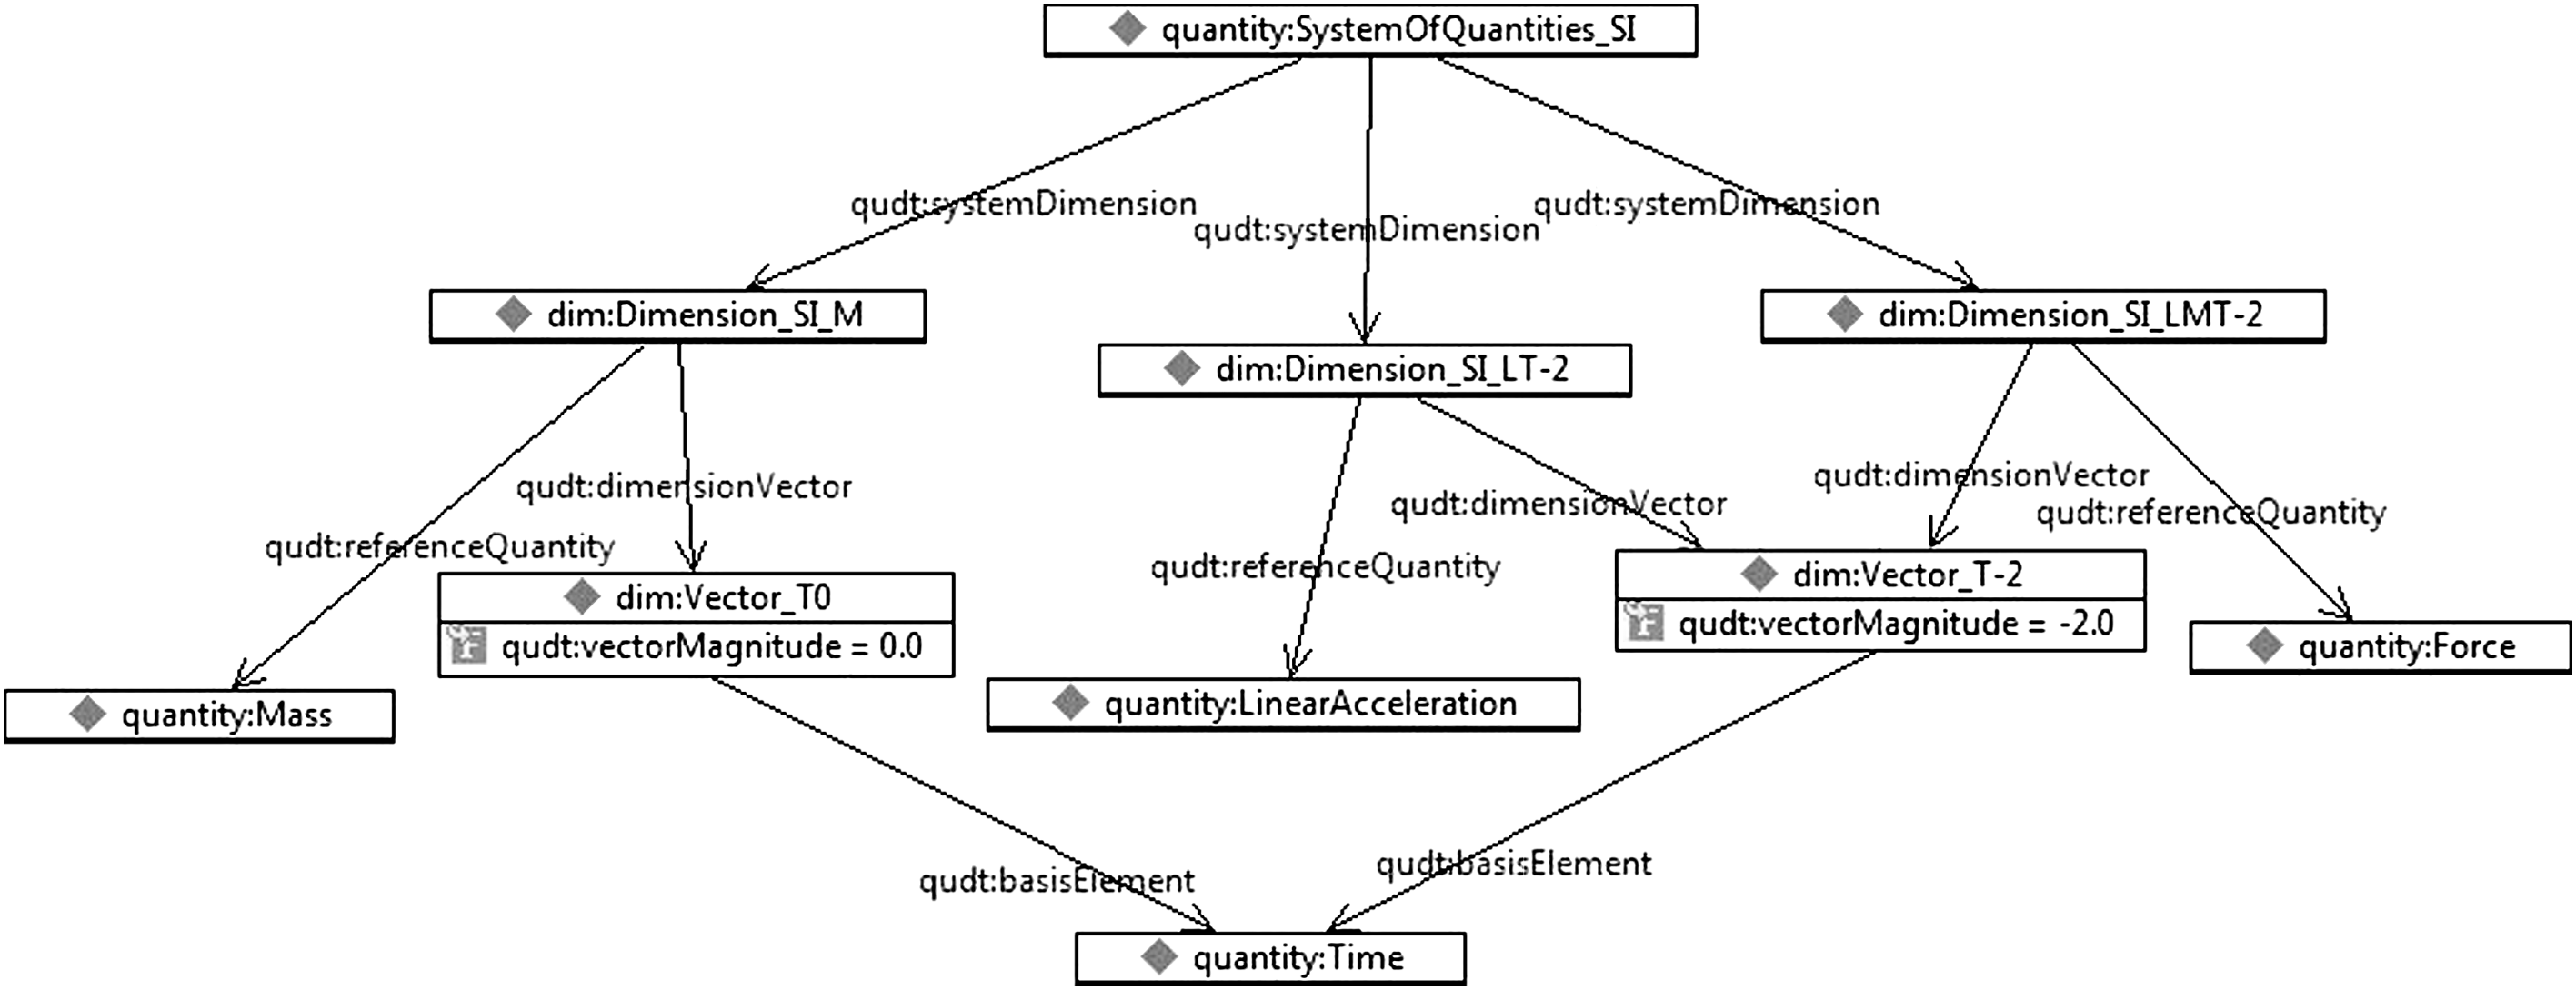
\includegraphics[width=5in]{media/ch14/f14-04.jpg}
\caption{Dimensional structure in QUDT to support analysis of F ¼ ma (time
dimension)}
\label{fig:ch14.04}
\end{figure}






QUDT supports dimensional analysis by representing over 200 dimensions,
cross-referenced with corresponding quantities. Figure~\ref{fig:ch14.04} shows the
structure in QUDT needed to support this sort of analysis. We will go
through each piece in turn.

First, there is the \emph{System of Quantities}. QUDT includes eight different
systems of quantities, including the standard international (``metric'')
system (SI, shown in the figure) as well as several variants of the CGS
(centimeter-gram-second) and the US Customary system (with inches,
yards, miles, pounds, etc.). A system of quantities defines the
dimensions that can be measured in that system. Each system typically
has dozens of dimensions associated with it. In the figure, we see three
dimensions associated with the SI system of quantities---one for mass
(\texttt{Dimension\_SI\_M}), one for length over time twice (\texttt{Dimension\_SI\_LT-2})
and one for length times mass over time twice (\texttt{Dimension\_SI\_LMT-2}).
The naming convention for these dimensions includes the name of the
system (SI) followed by the dimensions in the order length, mass, time,
each followed by a number indicating the exponent for that dimension.
These names are not used by any query mechanism---they are only used for
humans to read the dimension names.

Since the names are only there for humans to read, if we want to query
for the dimension vector for any of these, we need to represent their
dimensional vectors in triples. This is shown in Figure\ref{fig:ch14.05} for
\texttt{Dimension\_SI\_LMT-2}; for each of the three basis vectors, there is a
one-dimensional vector. The magnitude of the vector is given by the
property \texttt{vectorMagnitude} (its value is a floating point number, since
fractional exponents are possible for certain units). The base quantity
itself (mass, length, time) is given by the property \texttt{baseElement}.


\begin{figure}
\centering
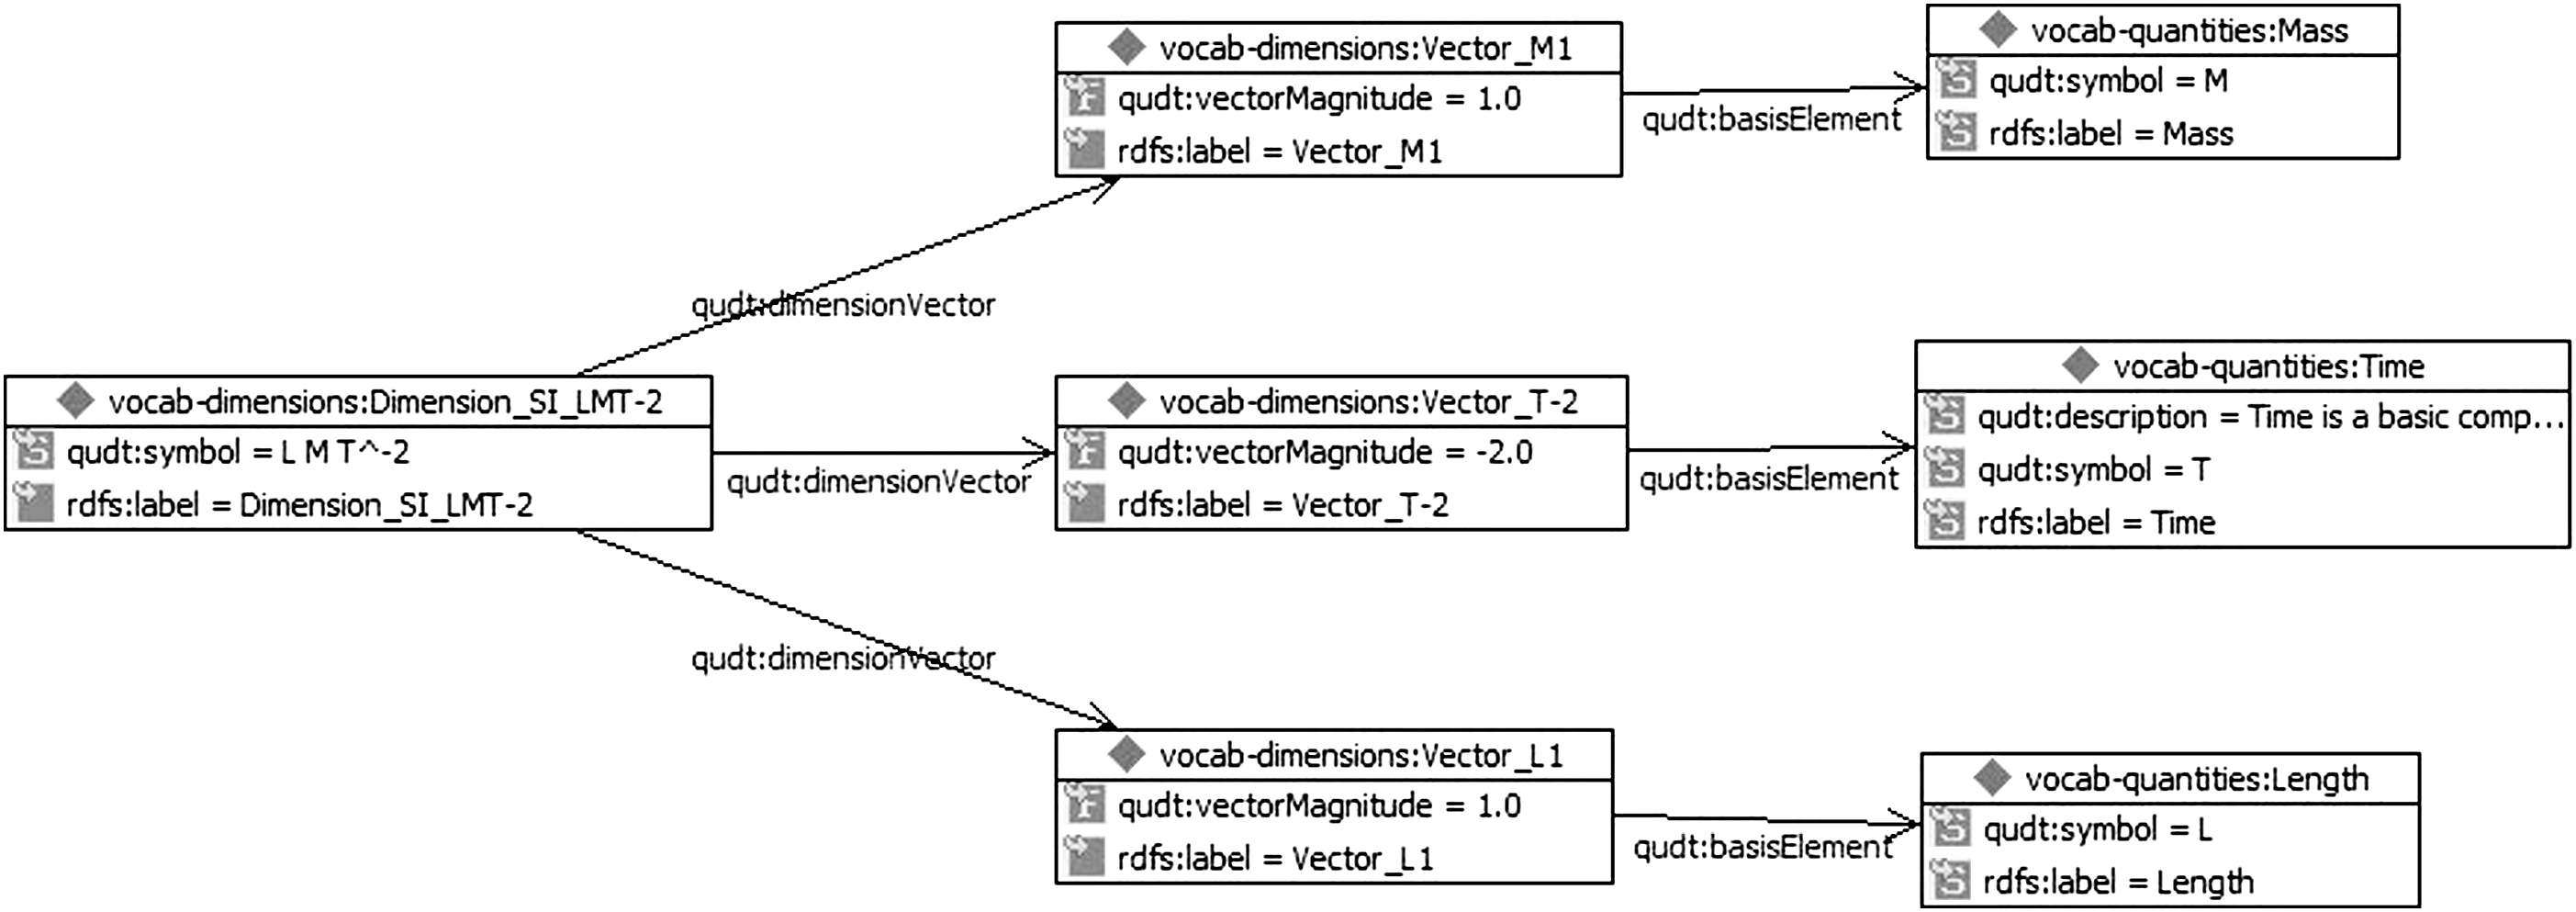
\includegraphics[width=5in]{media/ch14/f14-05.jpg}
\caption{QUDT dimensional breakdown of $ml/{t^2}$}
\label{fig:ch14.05}
\end{figure}

We can see all of this come together in Figure~\ref{fig:ch14.05} for the time
dimension; we have our three
quantities, \texttt{Mass}, \texttt{LinearAcceleration} and \texttt{Force}. Each of these is
referenced by a particular dimension expression -- $m$ for mass, $l/{t^2}$ for
linear acceleration, and $ml/{t^2}$ for force. Each of these, in turn, is
related to several base vectors. The figure shows the vector for time,
with coefficient zero for mass (since the vector for mass has a zero in
the time place), coefficient -2 for linear acceleration
(since the vector for linear acceleration has a -2 in the time place),
and also a coefficient -2 for force (since the vector for force also has
a -2 in the time place). From the information in Figure~\ref{fig:ch14.04}, we are in
a position to verify (for the time dimension, anyway) that the formula F
= ma is correct from a dimensional point of view, by noticing that the
time coefficient for mass (0) plus that for linear acceleration (-2)
equals the coefficient for force (-2); $0 + (-2) = -2$.

How can we write a SPARQL query to verify this calculation? First, let's
have a look at some of the information from Figure~\ref{fig:ch14.04} rendered
verbatim in Turtle:

\begin{lstlisting}
quantity:SystemOfQuantities_SI qudt:systemDimension dim:Dimension_SI_M .
dim:Dimension_SI_M qudt:referenceQuantity quantity:Mass .
dim:Dimension_SI_M qudt:dimensionVector dim:Vector_T0 .
dim:Vector_T0 qudt:vectorMagnitude "0.0"^{}^{}xsd:float .
dim:Vector_T0 qudt:basisElement quantity:Time .
\end{lstlisting}

We can use these triples to form a query that will tell us the magnitude
of the time dimension for the quantity mass by putting in variables at
the appropriate places:

\begin{lstlisting}
SELECT ?MassMagnitude
WHERE {
    quantity:SystemOfQuantities_SI qudt:systemDimension ?dim .
    ?dim qudt:referenceQuantity quantity:Mass .
    ?dim qudt:dimensionVector ?vector .
    ?vector qudt:vectorMagnitude ?MassMagnitude .
    ?vector qudt:basisElement quantity:Time .
}
\end{lstlisting}

Answer: 0.0

We can verify the correctness of the dimensionality of $F = ma$ by
repeating this pattern three times, once each for mass, acceleration and
force. If we filter with the formula (?MassMagnitude + ?AccMagnitude != ?ForceMagnitude), we will eliminate those dimensions
for which the vectors
don't add up.

If we replace \texttt{quantity:Time} with another variable (\texttt{?base}), we can repeat
this calculation for every vector base. We will need to list out those
bases; QUDT provides this list as the class \texttt{qudt:VectorBase}. Finally,
the dimension analysis matches exactly if there is no dimension for
which it fails. We accomplish this in SPARQL by putting the check for a
failure into a subquery, and then checking for no failures using the
SPARQL keyword NOT EXISTS. If there does not exist a failure, then the
query returns true. The complete query that checks the dimensions of $F = ma$ is shown here. It returns true, since the dimensions do check out.

\begin{lstlisting}
ASK WHERE
{
NOT EXISTS { SELECT *
WHERE { 
  ?base a qudt:VectorBase .
  quantity:SystemOfQuantities_SI  qudt:systemDimension ?dim1 .
  ?dim1 qudt:referenceQuantity quantity:Mass .
  ?dim1 qudt:dimensionVector ?vector1 .
  ?vector1 qudt:vectorMagnitude ?MassMagnitude .
  ?vector1 qudt:basisElement ?base .
  quantity:SystemOfQuantities_SI qudt:systemDimension ?dim2 .
  ?dim2 qudt:referenceQuantity quantity:LinearAcceleration .
  ?dim2 qudt:dimensionVector ?vector2 .
  ?vector2 qudt:vectorMagnitude ?AccMagnitude .
  ?vector2 qudt:basisElement ?base.
  quantity:SystemOfQuantities_SI qudt:systemDimension ?dim3 .
  ?dim3 qudt:referenceQuantity quantity:Force .
  ?dim3 qudt:dimensionVector ?vector3 .
  ?vector3 qudt:vectorMagnitude ?ForceMagnitude .
  ?vector3 qudt:basisElement ?base.
  FILTER (?MassMagnitude + ?AccMagnitude != ?ForceMagnitude)
} } }
\end{lstlisting}

The real test of a query like this is to try it on formulas that do not
check out. Indeed, if we replace e.g,. \texttt{Mass} with \texttt{Time} or \texttt{Force} with
\texttt{Energy} in this query, the result is false, since those dimensions do not
add up.

While it is easy enough to build up a query like this from identical
pieces, reading and maintaining them can become unwieldy. Since large
parts of the query are repetitive, this is a great opportunity to define
the repeating parts as SPIN functions. It is beyond the scope of this
book to work out all the dimensional analysis queries using SPIN---but
the same approach used to generate this query has been used to create
SPIN functions for checking the dimensionality of formulas. Details of
this approach can be found at http://qudt.org/.

\subsection{Summary}

QUDT is an elaborate ontology, but not a very large one. It includes a
few dozen classes and several hundred units, quantities, and vectors.
But it expresses subtle distinctions that are important for providing
services with units. It accomplishes the three major goals we laid out
at
the beginning of this section; it provides a global reference (URI) for
comprehensive systems of units, it provides a means for converting from
any unit to any commensurate unit, and it provides enough information to
perform dimensional analysis on any of over 200 units that it defines.
It accomplishes this with a careful separation of entities---quantities,
units and dimensions, as well as a comprehensive catalog of information
about the conventional units used throughout history and around the
world.

\section{Biological Ontologies}

Ontologies in one form or another have been a mainstay of biological and
life sciences for decades (one could even say for centuries). In recent
years, there has been an explosion of biological information, along with
a corresponding interest in ontologies to help organize that
information. In this ``in the wild'' study, we make no attempt to
provide a comprehensive catalog of biological ontologies. We will
instead concentrate by example on the modeling aspects of biomedical
ontologies and their use in the Semantic Web.

Just as was the case with QUDT, the biological ontologies serve many
purposes on the Semantic Web. First, they provide unambiguous references
to biological concepts. This is particularly important when there are
tens of thousands of relevant concepts, including information about
genes, diseases, chemicals, and organisms, etc. Having unambiguous names
of this sort is essential for organizing information generated in
different laboratories. Unambiguous terms of this sort are essential for
locating publications---if a researcher suspects something interesting
about a particular gene, indexing the vast corpus of biological
publications for appropriate material is considerably enhanced by
unambiguous names.

A closely related function has to do with the observation that in any
global endeavor, many people will have already come up with naming
schemes for these things---there are already multiple naming schemes for
proteins, chemicals, and other biological entities. A key role of many
of the biological ontologies is to provide a sort of Rosetta Stone to
link these vocabularies together. The Semantic Web is a particularly
suitable infrastructure for this sort of interoperation of vocabularies.

A more involved use of a biological ontology is for solving elaborate
search problems, where the search relies on massive amounts of detailed
knowledge about a technical domain (like chemistry, genomics, and
proteomics). This places much more stringent requirements on an
ontology. Many of the ontologies published today have sufficient detail
to satisfy these requirements.

In this exposition, we will use an ontology called the Chemical Entities
of Biological Interest (CHEBI, for short). CHEBI is being developed and
maintained by the European Bioinformatics Institute, and contains
information about over 20,000 chemical compounds. It is published as
part of the Open Biological and Biomedical Ontologies Foundry (OBO
Foundry), a sort of wiki space for collecting science-based ontologies.
The OBO Foundry publishes ontologies in a number of forms including OWL.
OBO Foundry OWL ontologies use certain ontology design patterns that we
will examine in detail.

\subsection{CHEBI as Unambiguous Reference}

CHEBI provides a URI identifier for every chemical it defines, and hence
serves as a global reference for those chemicals. But CHEBI is not the
only resource that identifies chemicals---many other
resources do this as well. These other resources do not necessarily
share CHEBI's focus on chemicals of biological interest, but there is
still considerable overlap. For this reason, CHEBI includes several
cross-references for each chemical it defines. For example, the
herbicide glyphosate (better known by its trade name, Roundup) is
represented in CHEBI as

\begin{lstlisting}
chebi:CHEBI_27744
    rdfs:label "glyphosate"@en ;
    oboInOwl:hasDbXref
       [ a oboInOwl:DbXref ;
         rdfs:label "ChemIDplus:1071-83-6"
       ] ;
    oboInOwl:hasDbXref
       [ a oboInOwl:DbXref ;
         rdfs:label "KEGG_COMPOUND:1071-83-6"
       ] ;
    oboInOwl:hasDbXref
       [ a oboInOwl:DbXref ;
         rdfs:label "Beilstein:2045054"
       ] ;
    oboInOwl:hasDbXref
       [ a oboInOwl:DbXref ;
         rdfs:label "MSDchem:GPJ"
       ] ;
    oboInOwl:hasDbXref
       [ a oboInOwl:DbXref ;
         rdfs:label "Gmelin:279222"
       ] .
\endlstlisting

Glyphosate has identifying number 27744 in CHEBI, which is actually
represented as the URI \texttt{Chebi:CHEBI\_27744}. Every entity in CHEBI is
assigned a number like this. While this policy makes the URIs difficult
to read, it makes them easier to use in a multi-lingual setting or, as
in this case, in a setting in which multiple names could be preferred by
different groups. In defining cross- references to other chemical
identification systems, CHEBI makes ample use of reification (Chapter
3). Each cross-reference is an individual member of the class
\texttt{oboInOwl:DbXref}, with a label that indicates the details of the
reference. In the example, we see references to several other
authorities, with names given in the references (ChemIDPlus, Kegg,
etc.). The DbXref is reified to allow other information to accompany the
cross reference as available, e.g., a pointer to the governing body,
effective dates, etc. This structure allows CHEBI to act as a sort of
translation service among these other resources, for the chemicals that
it describes.


\subsection{CHEBI for Complex Search}

A good deal of the complexity of the CHEBI ontology lies in the
connections between the chemicals. It is typical of OBO ontologies to
include complex interrelationships between the entities they define.
CHEBI makes a particularly good pedagogical example of OBO style because
of its relatively small size (only 20,000 concepts) and the small number
of relationships between the chemicals it records.

Using our example chemical glyphosate, the fact that it is an herbicide
is represented in CHEBI as

\begin{lstlisting}
chebi:CHEBI_24527
     a owl:Class ;
     rdfs:label "herbicide"@en .
chebi:CHEBI_27744
     a owl:Class ;
     rdfs:label "glyphosate"@en ;
     rdfs:subClassOf
     [ a owl:Restriction ;
       owl:onProperty obo:has_role ;
       owl:someValuesFrom chebi:CHEBI_24527
     ] ;
\end{lstlisting}


The first thing to notice in this style of modeling is that every
concept is represented in OWL as an \texttt{owl:Class}; the chemical
``glyphosate'' (\texttt{Chebi:CHEBI\_27744}) as well as the role ``herbicide''
(\texttt{Chebi:CHEBI\_24527}) are both classes. These two classes are related to
one another as shown; glyphosate is a subclass of an \texttt{owl:Restriction} (as
defined in Chapter\ref{ch11}), where that restriction is on the property
\texttt{obo:has\_role}, and stipulates that this property takes at least one
value from (\texttt{owl:someValuesFrom}) the class herbicide. Notice that the
property \texttt{obo:has\_role} comes from OBO namespace; OBO Foundry defines
dozens of prop- erties that are useful for describing biological
entities. CHEBI uses less than a dozen of them that have relevance to
its domain of biochemistry. In addition to \texttt{obo:has\_role} seen in this
example, CHEBI uses \texttt{obo:has\_part} (for constituent chemicals), and
several chemistry-specific properties like \texttt{obo:is\_conjugate\_acid\_of},
\texttt{obo:is\_conjugate\_base\_of}, and \texttt{obo:has\_parent\_hydride}. The pattern
we see here with \texttt{has\_ role} and \texttt{herbicide} is repeated in CHEBI
about 12,000 times, to relate various chemicals to their components,
conjugate acids and bases, parent hydrides, etc. This pattern is typical
of OBO ontologies and is used thousands of times in OBO Foundry.

Since this pattern is being used to reflect the fact that glyphosate has
the role of herbicide, one might well wonder why this wasn't represented
simply with a single triple

\begin{lstlisting}
chebi:CHEBI_27733 obo:has_role chebi:CHEBI_24527 .
\end{lstlisting}

As usual, the answer to a question like this lies in the inferencing.
What inferences can we draw from this pattern?

To see the answer to this, we need to view glyphosate in a larger
context. Figure~\ref{fig:ch14.06} shows some of the context of glyphosate in CHEBI.

CHEBI goes into considerable detail about classifications of chemicals.
We see in this figure the information about glyphosate's role as an
herbicide (center). It is a subclass of a restriction on the property
\textit{has role} that takes some value from the class \textit{herbicide}. But we have
further context about herbicide, in particular that it is a subclass of
\textit{pesticide}. We also see that \textit{glyphosate} is a subclass, through a long
chain of intermediaries, of two more restrictions, which stipulate that
for\textit{ has part} it takes some value from \textit{phosphorus}, and that for\textit{ has
parent hydride}, it takes some value from \textit{ammonia}.


\begin{figure}
\centering
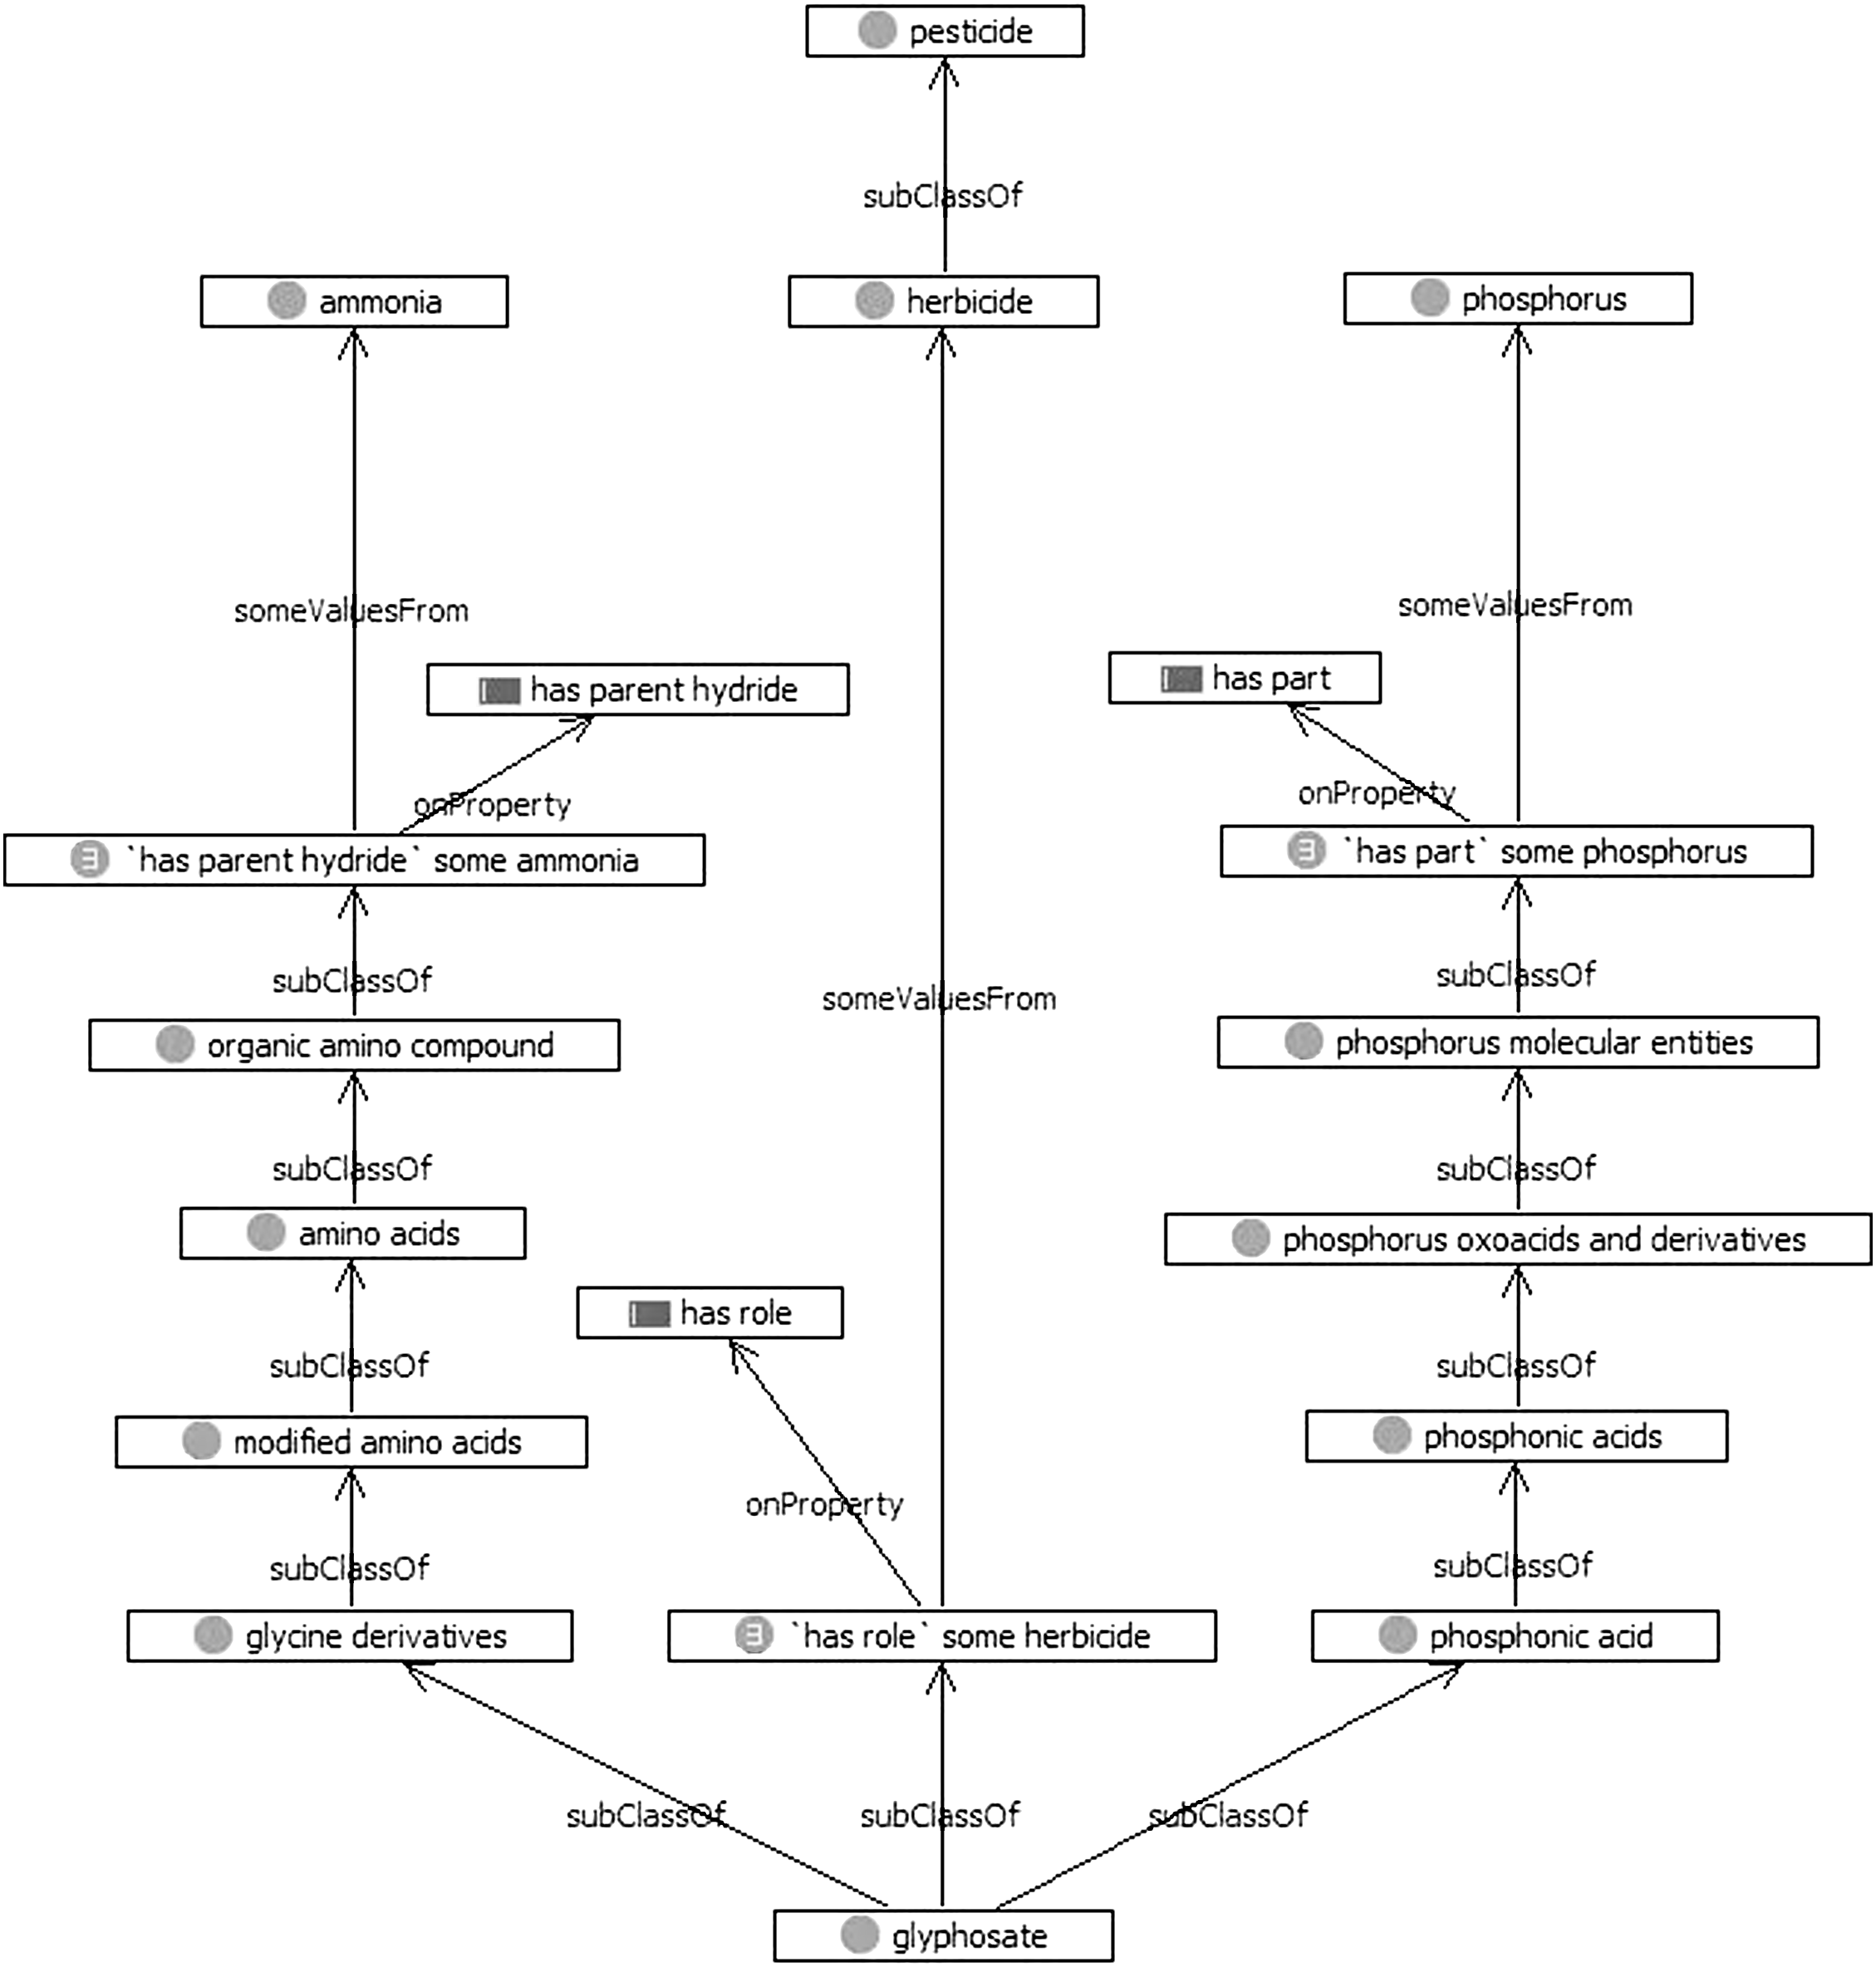
\includegraphics[width=5in]{media/ch14/f14-06.jpg}
\caption{Excerpt from CHEBI, showing information about glyphosate. All concepts
are shown with labels (e.g., ``glyphosate'') instead of CHEBI URIs
(e.g., \texttt{Chebi:CHEBI\_27744}).
}
\label{fig:ch14.06}
\end{figure}

Given these facts, we can use the inference mechanism of OWL to answer
some useful questions. Suppose we are interested in pesticides
containing phosphorus that have ammonia as a parent hydride. Figure
13.6, along with an understanding of the meaning of the modeling words
\texttt{rdfs:subClassOf}, \texttt{owl:someValuesFrom}, and \texttt{owl:onProperty} tells us that
glyphosate is such a chemical. But how, specifically, can we find this
(or any other such chemical), based on this model?

First, we define (in OWL) the class of things we are seeking, that is,
the intersection of things that have \textit{role} pesticide, have \textit{part}
phosphorus, and have \textit{parent hydride} ammonia. This is done with an
intersection of three restrictions. (In RDF, we have to use the CHEBI
URIs to refer to concepts; for reference, we have included the
corresponding names of the concepts pesticide, ammonia and
phosphorus in comments indicate with a hash (\#) on each line where they
occur.) Here's how that looks:

\begin{lstlisting}
:MyChemical a owl:Class ;
    rdfs:label "My chemical" ;
    owl:intersectionOf
       (
         [ a owl:Restriction ;
           owl:onProperty obo:has_role ;
	   owl:someValuesFrom chebi:CHEBI_25944 ] # pesticide
         [ a owl:Restriction ;
	   owl:onProperty obo:has_parent_hydride ;
	   owl:someValuesFrom chebi:CHEBI_16134 ] # ammonia
         [ a owl:Restriction ;
	   owl:onProperty obo:has_part ;
	   owl:someValuesFrom chebi:CHEBI_28659 ] # phosphorus
) .
\end{lstlisting}

Now if we run OWL inferences, we infer that

\begin{lstlisting}
chebi:CHEBI_27733 rdfs:subclassOf :MyChemical .
\end{lstlisting}

That is, \textit{glyphosate} is a match for the given specifications. The OWL
semantics took care of all the complexity of Figure~\ref{fig:ch14.06}, including the
chain of named classes that \textit{glyphosate} is a subclass of, as well as the
subclass chain between its stated role \textit{herbicide} and the required role
\textit{pesticide}. The definition of the requirements didn't include any
reference to any of these things---that was included in the CHEBI model
and the OWL semantics.

It is also worth noting what inferences we \textbf{\textit{cannot}} draw from the CHEBI
model as shown in Figure~\ref{14.06}. If, for example, we have a sample
chemical in our lab, and our experiments show that it contains
phosphorus as a part, and has ammonia as a parent hydride, this allows
us to infer its membership in the two corresponding restrictions at the
top of Figure~\ref{14.06}. But this does not allow us to infer anything about
the relationship of our sample to \textit{glyphosate}. CHEBI is useful for
searching for chemicals among those classified within it, not for
identifying samples.

These examples provide some motivation for why the authors of CHEBI
chose to define the
herbicide role of glyophosate as a relationship between classes using
someValuesFrom, rather than simply stating it as an explicit fact in a
single triple.

\begin{lstlisting}
chebi:CHEBI_27733 obo:has_role chebi:CHEBI_24527 .
\end{lstlisting}

By modeling this relationship with classes and \texttt{someValuesFrom}, they
embedded the class \textit{glyphosate} in a more comprehensive model that
includes relevant facts, for example, facts about the relations between
pesticides and herbicides. This allows the model (along with the OWL
semantics) to do a lot of the work of question answering (for certain
questions) about the entities in the model. The model encodes
information in a way that a human questioner need not be aware of.

\begin{challenge}{Expressing CHEBI in SKOS}
\label{chal:39}

The power of a model like CHEBI to respond flexibly to queries like this
one comes at a price---the model itself is complex; for example, the
relationship between \textit{glyphosate} and \textit{herbicide} is given by a pattern
including a particular kind of restriction. Earlier, we asked why this
couldn't have been represented simply with a single triple

\begin{lstlisting}
chebi:CHEBI_27733 obo:has_role chebi:CHEBI_24527 .
\end{lstlisting}

In this challenge, we will examine how CHEBI could be represented in
SKOS, and how we could satisfy the same information extraction needs
outlined above, using that representation.

In the case of CHEBI, it is a simple matter to convert all the
information about subclasses and restrictions into SKOS following this
line of reasoning. Each class in CHEBI becomes a SKOS concept, each
\texttt{rdfs:subClassOf} relationship becomes \texttt{skos:broader}, and each
\texttt{owl:someValuesFrom} restriction becomes a direct reference. Figure\ref{fig:ch14.07}
shows the same information from Figure~\ref{14.06}, but transformed into SKOS
in this way.

In many ways, Figure~\ref{14.07} is simpler than Figure Figure~\ref{14.06}; the fact that
glyphosate has role herbicide is represented as a single triple, as is
the fact that an organic amino compound has parent hydride ammonia. The
inclusion relationships that were expressed as \texttt{subClasbsof} are now
expressed as \texttt{broader}. But how would we query this structure to find an
answer to the same question we asked earlier---``find the pesticides
containing phosphorus that have ammonia as a parent hydride''? We can
find these using SPARQL as follows:

\begin{lstlisting}
SELECT ?result
WHERE {
  ?result skos:broader* ?concept1 .
  ?concept1 obo:has_parent_hydride ?concept2 .
  ?concept2 skos:broader* chebi:CHEBI_16134 . # ammonia
  ?result skos:broader* ?concept3 .
  ?concept3 obo:has_part ?concept4 .
  ?concept4 skos:broader* chebi:CHEBI_28659 . # phosphorus
  ?result skos:broader* ?concept5 .
  ?concept5 obo:has_role ?concept6 .
  ?concept6 skos:broader* chebi:CHEBI_25944 . # pesticide
}
\end{lstlisting}

This gives the same result as the OWL inference, namely that \textit{glyphosate}
satisfies all of these criteria. The representation is simpler, but the
query is more complex. In particular, the query writer must take
responsibility for all of the transitive relationships, using
\texttt{skos:broader}* at each point, and making sure that it appears at every
point in the query. This is a common trade-off in representation---does
the model do more work, with a more involved representation, or does the
query do more work, matching the correct information? The contrast
between the OWL version of CHEBI and the SKOS version shows this; in
OWL, certain queries can be done very easily, allowing the structure of
the model to do all the work. But the structure is less suited to other
queries (``Identify this sample''). The model does more of the work for
the queries it was designed for, but its increased complexity can make
other applications more complex.

The transformation from OWL into SKOS shown here was straightforward,
because CHEBI uses a single pattern (using \texttt{owl:someValuesFrom}) to relate
one concept to another. Some models use more complex pattern in OWL to
relate concepts. For instance, one of the OBO Foundry ontologies is a
thesaurus of cancer entities maintained by the National Cancer Institute
(NCI). The NCI thesaurus includes disease descriptions (with far too
much technical detail to include here) in which a disease is
characterized by several syndromes---that is, a particular disease is
indicated by a certain set of symptoms or another set of symptoms or
another set of symptoms and so on. Complicated combinations of unions
and intersections can be done in OWL in a standard way; the translation
to SKOS of such things is not straightforward. An OWL inference engine
will treat all such definitions in a consistent and correct manner.



\begin{figure}
\centering
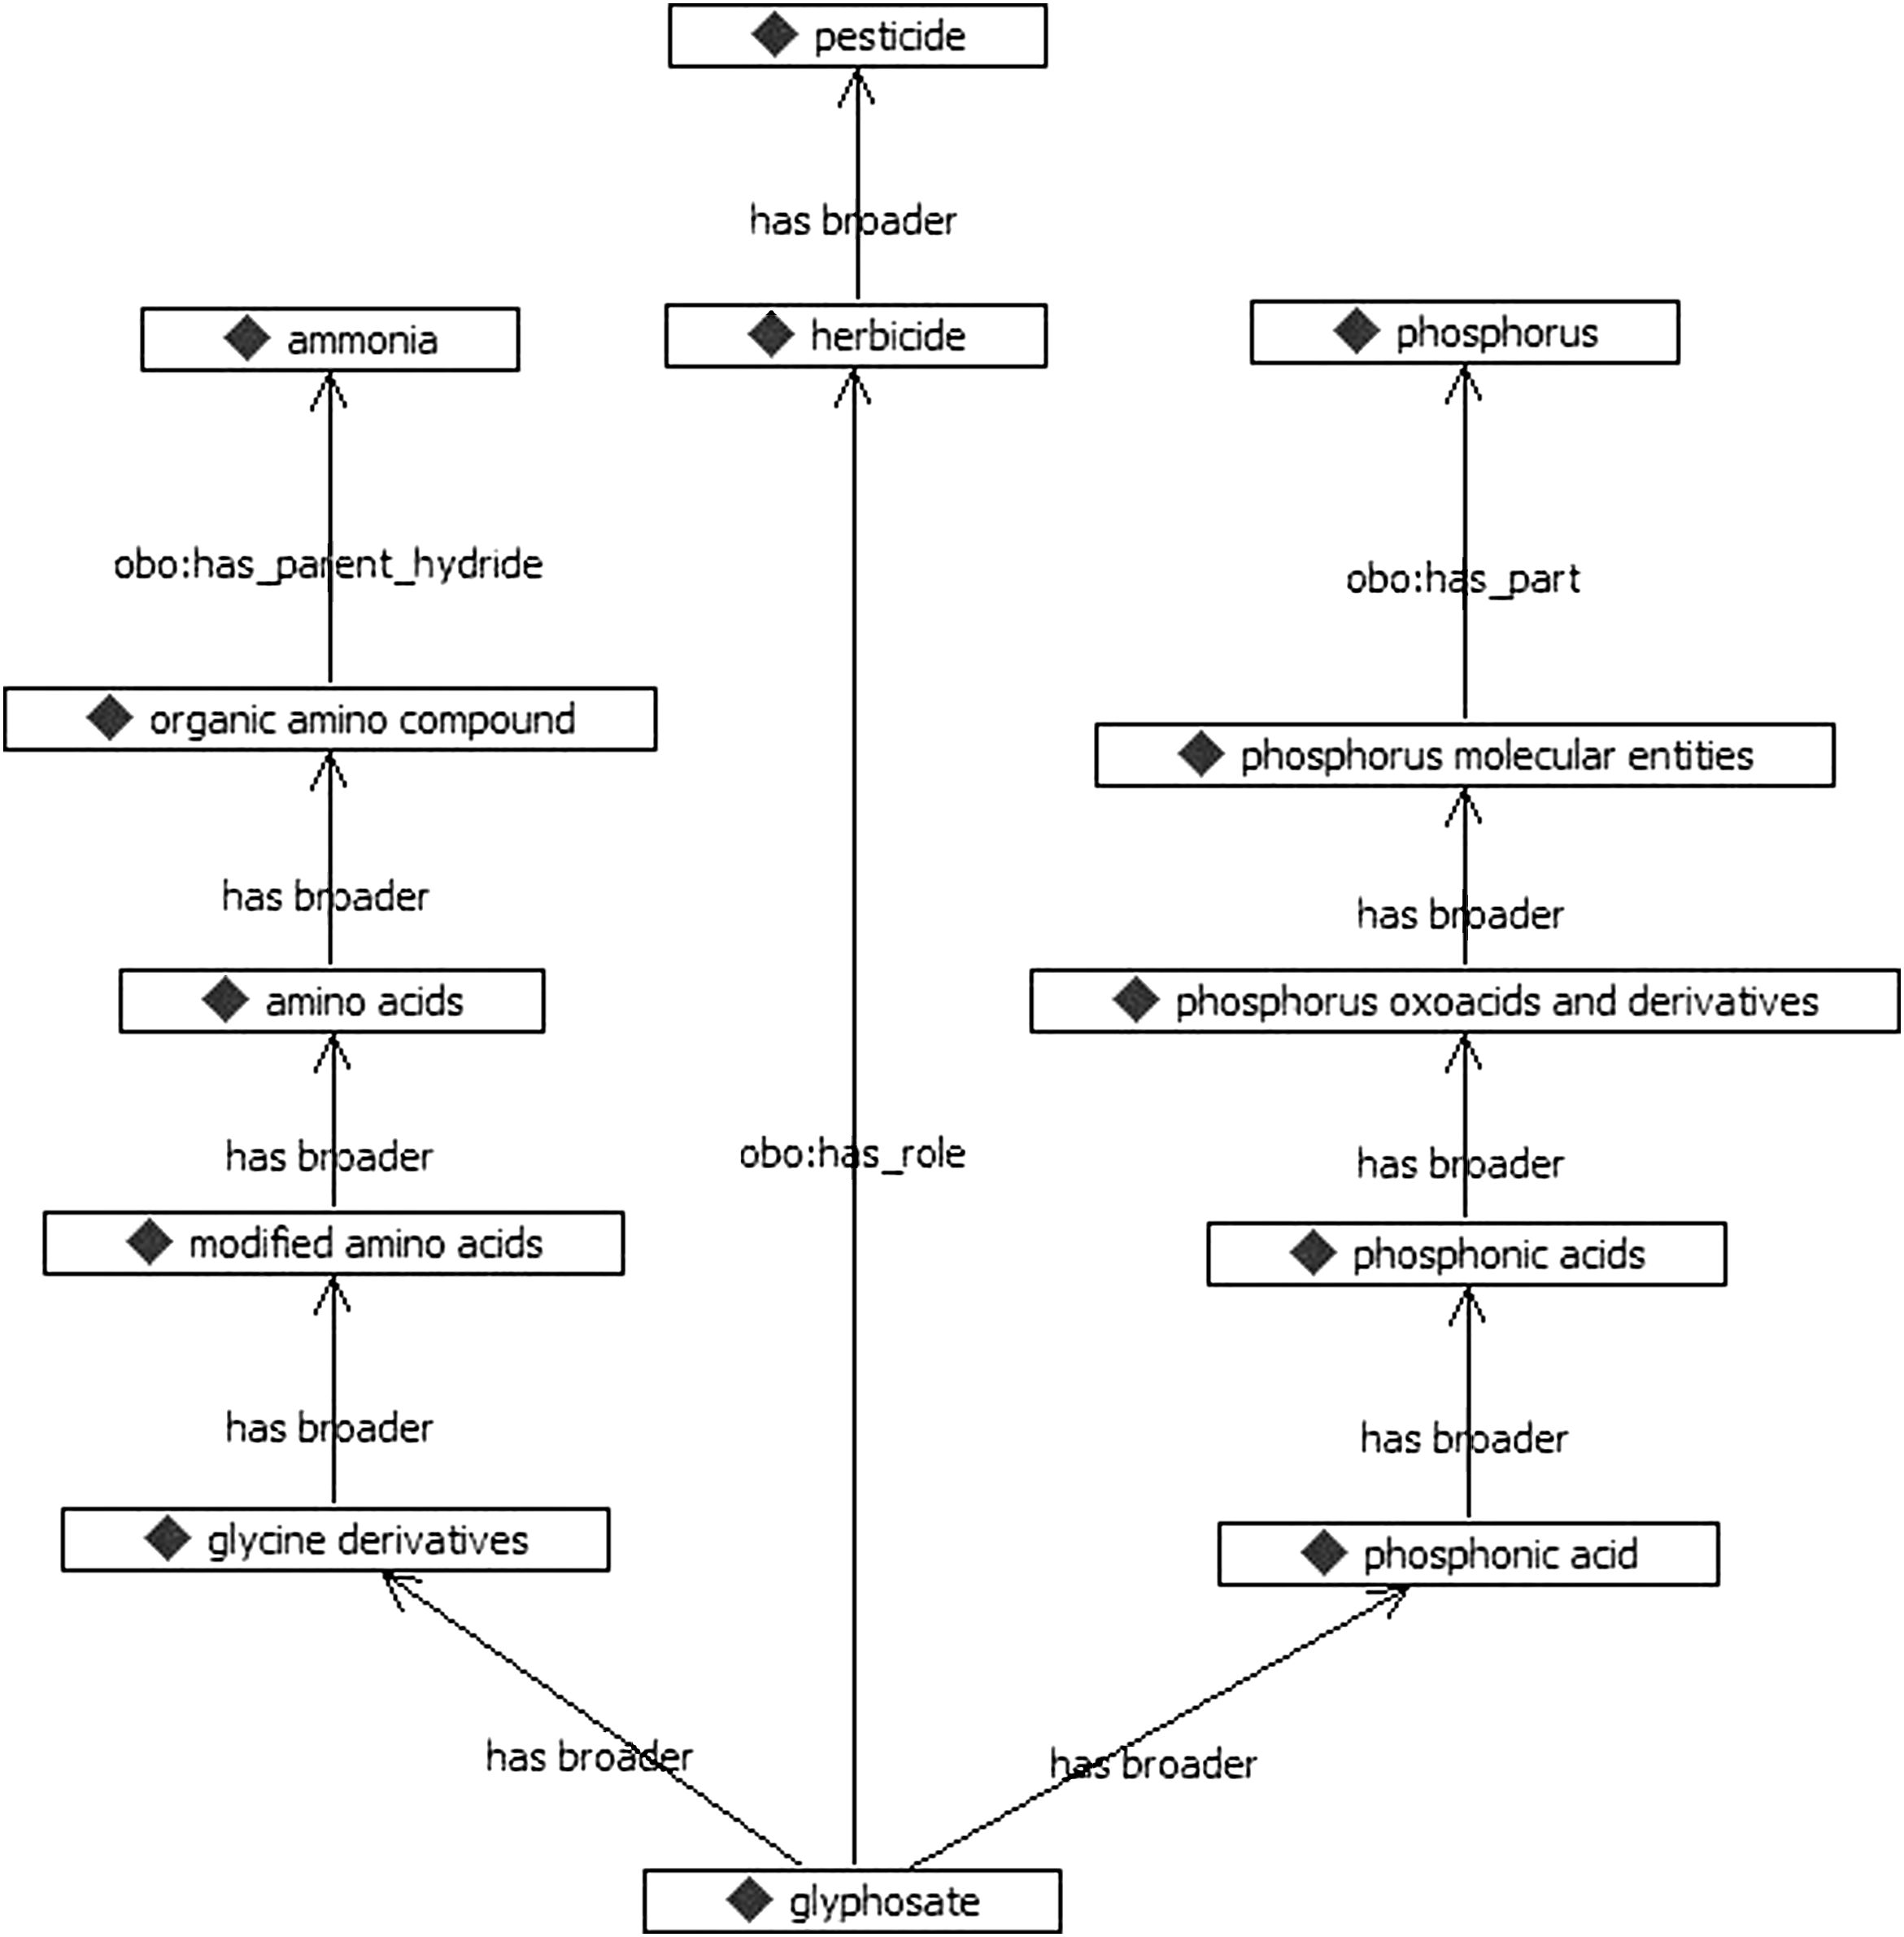
\includegraphics[width=5in]{media/ch14/f14-07.jpg}
\caption{CHEBI concepts from Figure 13.6 shown in SKOS. The standard SKOS
property \texttt{skos:broader} is shown here as ``has broader.''
}
\label{fig:ch14.07}
\end{figure}


\section{SUMMARY}

The three ontologies discussed in this chapter, Good Relations, QUDT,
and OBO Foundry ontologies, cover the spectrum from ontologies that
include almost no data at all (Good Relations) to ontologies that
include very large amounts of richly interconnected data (OBO). They all
supply, to varying extents, the basic capabilities of the Semantic Web
of sharing information in a coherent way across multiple systems.

Good Relations is the smallest of the ontologies described here. Its
main goal in the Semantic Web is to provide a framework in which
information can be shared---a vocabulary that different suppliers
can use to describe their offerings. The data in Good Relations aren't
in the ontology at all; it is distributed across the Web. OBO Foundry
ontologies, in contrast, are much, much larger, and include large
amounts of data about biology, medicine, life sciences, etc. There are
complex questions that can be answered, using OBO as a data resource.
QUDT sits in the middle; it contains a good deal of data (conversion
factors, relationships between dimensions and units, etc.), but its main
purpose is to provide connection between other data sets; two data
sources that both use Good Relations might still fail to be
interoperable because of mismatch of units; QUDT provides enhanced
interoperability in these cases. All three of these ontologies play the
basic role in the Semantic Web of providing globally unambiguous names
for standard entities---they differ only in the details of how these
relationships can be used.

\subsection{Fundamental concepts}

The following fundamental concepts were introduced in this chapter.

owl:imports---Allows one ontology to refer explicitly to another.
Triples from the imported ontology are available for inferencing in the
importing ontology.

Ontology Design Patterns---Repeated modeling idioms that provide
coherence and unity to a large model.

Good Relations---Ontology for representing and sharing information about
commerce on the Web.

QUDT---Quantities, Units, Dimensions Types. Ontology of engineering
units

OBO---Open Biological and Biomedical Ontologies. A collection of
ontologies with relevance to the life sciences.

CHEBI---Chemical of Biological Interests. An example ontology from OBO
relating to biochemistry.
